%%%%%%%%%%%%%%%%%%%%%%%%%%%%%%%%%%%%%%%%%%%%%%%%%%%%%%%%%%%%%%%%%%%%%%%%%%%%%%%%
% Template for USENIX papers.
%
% History:
%
% - TEMPLATE for Usenix papers, specifically to meet requirements of
%   USENIX '05. originally a template for producing IEEE-format
%   articles using LaTeX. written by Matthew Ward, CS Department,
%   Worcester Polytechnic Institute. adapted by David Beazley for his
%   excellent SWIG paper in Proceedings, Tcl 96. turned into a
%   smartass generic template by De Clarke, with thanks to both the
%   above pioneers. Use at your own risk. Complaints to /dev/null.
%   Make it two column with no page numbering, default is 10 point.
%
% - Munged by Fred Douglis <douglis@research.att.com> 10/97 to
%   separate the .sty file from the LaTeX source template, so that
%   people can more easily include the .sty file into an existing
%   document. Also changed to more closely follow the style guidelines
%   as represented by the Word sample file.
%
% - Note that since 2010, USENIX does not require endnotes. If you
%   want foot of page notes, don't include the endnotes package in the
%   usepackage command, below.
% - This version uses the latex2e styles, not the very ancient 2.09
%   stuff.
%
% - Updated July 2018: Text block size changed from 6.5" to 7"
%
% - Updated Dec 2018 for ATC'19:
%
%   * Revised text to pass HotCRP's auto-formatting check, with
%     hotcrp.settings.submission_form.body_font_size=10pt, and
%     hotcrp.settings.submission_form.line_height=12pt
%
%   * Switched from \endnote-s to \footnote-s to match Usenix's policy.
%
%   * \section* => \begin{abstract} ... \end{abstract}
%
%   * Make template self-contained in terms of bibtex entires, to allow
%     this file to be compiled. (And changing refs style to 'plain'.)
%
%   * Make template self-contained in terms of figures, to
%     allow this file to be compiled. 
%
%   * Added packages for hyperref, embedding fonts, and improving
%     appearance.
%   
%   * Removed outdated text.
%
%%%%%%%%%%%%%%%%%%%%%%%%%%%%%%%%%%%%%%%%%%%%%%%%%%%%%%%%%%%%%%%%%%%%%%%%%%%%%%%%

\documentclass[letterpaper,twocolumn,10pt]{article}
\usepackage{usenix2019_v3}

% to be able to draw some self-contained figs
\usepackage{tikz}
\usepackage{amsmath}

%\usepackage{natbib} 
\usepackage{comment}

% inlined bib file
%\usepackage{filecontents}

\usepackage{todonotes}
\newcommand{\marcos}[1]{\todo[author=Marcos,inline]{#1}}
\newcommand{\barath}[1]{\todo[author=Barath,inline]{#1}}

\usepackage{xspace}
\newcommand{\system}{eBPFlow\xspace}

\microtypecontext{spacing=nonfrench}



%-------------------------------------------------------------------------------
\begin{document}
%-------------------------------------------------------------------------------

%don't want date printed
\date{}

% make title bold and 14 pt font (Latex default is non-bold, 16 pt)
\title{\Large \bf eBPFlow: Turing-Complete Hardware Packet Processing}

%for single author (just remove % characters)
\author{
{\rm Your N.\ Here}\\
Your Institution
\and
{\rm Second Name}\\
Second Institution
% copy the following lines to add more authors
% \and
% {\rm Name}\\
%Name Institution
} % end author

\maketitle


\begin{abstract}
%The OpenFlow standard is the most used solution in SDN, separating the data plane from the control plane and using a limited set of fields and actions. However, OpenFlow does not allow to include new fields outside the specification, making it difficult to adopt new protocols and services.
Providing an expressiveness (Turing-Complete) abstraction for network function packet processing in hardware remains a research challenge. 
In this work, we propose eBPFlow, a hardware-implemented packet processing that is Turing-Complete. It enables to program stateful and stateless network functions.
It also enables the use of dynamically defined new fields and protocols, without the need to recompile or restart the hardware platform when the user changes, at run time, how the flows should be processed. 
eBPFlows run an eBPF (enhanced Berkeley Packet Filter) processor that enables the processing of protocol-independent network flows using eBPF instructions generated from programs created by the user written in high-level languages.
Our prototype was implemented on the NetFPGA SUME 40 Gb/s platform.
We show the feasibility of building network functions, such as learning switch, load balancers, and cryptography function. 
Our results show that the system allows modifying parsing, matching, and actions at run time with zero downtime.
eBPFlow implementation is publicly available.
\end{abstract}

%As an initial instance, we measure the throughput for different packet sizes in a real-world environment. 


\section{Introduction}
\label{sec:intro}

Software-Defined Networking (SDN) is a paradigm for the development of research in computer networks that has gained the attention of the scientific community and industry in the area. SDN is a paradigm that separates the control plane from the data plane and allows the administrator to program the devices~\cite{ProgrammableNetworks2015}. In SDN, the control plane configures the routing rules of the network with a logically centralized entity called controller, while the data plane forwards the packets according to the actions defined by this controller. Due to the structure that SDN provides, research areas such as traffic engineering, quality of service (QoS), and virtualization have evolved rapidly~\cite{stubbe2017p4}.

The OpenFlow~\cite{McKeown:2008:OpenFlow} standard is an example of SDN, which has seen significant growth since its first release in 2008 until the release of the current version (1.5)~\cite{ChristianSurveySDN2015}. The first version of OpenFlow had a matching table of ten fields and evolved into multiple tables with 44 different fields~\cite{ChristianSurveySDN2015}. However, the number of fields supported by OpenFlow is constantly being updated to support new fields and protocols, such as the IPv6 protocol. Unfortunately, OpenFlow has a protocol-dependent data plane with parsing, matching, and fixed actions, making it difficult to support new fields and protocols~\cite{Jouet:2017:BPFabric}.

A protocol-independent switch is a device that does not have the protocol specification a priori. It does not know how to process a specific protocol until the programmer tells how to do it. The switch works as a substrate to process packets but it is not tied to a given protocol. Protocol-independent switch enables including recent protocols such as NVGRE~\cite{rfc7637}, VxLAN~\cite{mahalingam2013}, STT~\cite{davie2014stt}, PBB~\cite{kishjac-bmwg-evpntest-08}, OTV~\cite{hasmit-otv-04}, GENEVE~\cite{ietf-nvo3-geneve-05}, and NSH~\cite{rfc8300} without hardware modification.
% It also permit to customize what protocols to process. For instance, Amazon Virtual Private Cloud (VPC) was reported to only performs unicast IPv4 forwarding~\cite{Amazon2013Pepelnjak}. Thus, data center providers can benefit from protocol-independent switches by customizing only the necessary protocols they need for packet processing.

PISCES~\cite{Shahbaz:2016:Pisces} is a software protocol-independent switch that overcomes some of the OpenFlow limitations by permitting relational comparison with >, <, and logical operator and. The P4-to-OVS compiler in PISCES outputs C source code that replaces
the parsing, match, and action code in OVS~\cite{Pfaff:2015:OpenVSwitch}. But, to change the functionality of the switch, PISCES requires to recompile the software switch and reinstall it.

Moreover, hardware devices give the impression of being inflexible since their components are hard-coded and hard-placed. We address the following question: Is it possible to design a programmable protocol-independent hardware switch that enables to modify the parsing, matching, and actions at runtime? 

 \begin{figure}[!htp]
 \centering
\includegraphics[width=.8\linewidth]{figures/"eBPFlow Design Space".pdf}
 \caption{Design Space}
 \label{fig:03architecture}
 \end{figure}

%\textcolor{blue}{Add eBPF explanation}

This work proposes eBPFlow, a switch implemented in hardware, that allows the utilization of new dynamically defined fields and protocols, without the need to recompile or restart the switch when the user changes at run time how the flows should be processed. 
eBPFlow leverages eBPF (enhanced Berkeley Packet Filter), a bytecode machine and protocol independent instruction set. % to define parsing, matching, and functionalities of the data plane.
The switch was prototyped on the NetFPGA SUME 40 Gb/s~\cite{SUME2014} platform. The tests were performed in a real environment. eBPFlow allows to parse, match, and make actions in the data plane at runtime with zero downtime.

%\textcolor{blue}{vantagem de zero downtime}
Zero downtime is important to provide services without interruptions.
Google~\cite{Jain:2013:BEG:2486001.2486019} reported a substantial outage when doing maintenance. In  Amazon's platform Dynamo~\cite{DeCandia:2007:DAH:1294261.1294281},  services have stringent requirements to meet the customer's Service Level Agreements (SLA).
An outage can mean lost of money for not providing the service or even real lost sales on e-commerce sites.



The main contributions of this work are: (i) to permit the use of new dynamically defined fields and protocols without the need to recompile or restart the switch when the user changes at run time how the flows are to be processed; (ii) processing protocol-independent network flows using eBPF instructions generated from user-created C or P4 language programs; (iii) logic design and implementation of eBPFlow, a network hardware switch that includes the eBPF processor. Our system allows changing the parse, matching, and actions at run time with zero downtime. We emphasize that all these contributions together are not possible in other systems, such as BPFabic~\cite{Jouet:2017:BPFabric}, PISCES~\cite{Shahbaz:2016:Pisces}, P4FPGA~\cite{p4fpga}, RMT~\cite{bosshart2013forwarding}, and dRMT~\cite{chole2017drmt}. 

This paper is organized as follows. In \textsection\ref{sec:architecture}, we present the overall architecture of eBPFlow. In \textsection\ref{sec:design}, we provide the eBPFlow switch design. In \textsection\ref{sec:implementation}, we describe the implementation details of the eBPFlow switch at the NetFPGA platform. In \textsection\ref{sec:results}, we show the evaluation and results in a realistic environment. 
In \textsection\ref{sec:discussion}, we provide some analysis and discuss some limitations.
In \textsection\ref{sec:relatedWork}, we describe and compare the related work. Finally, in \textsection\ref{sec:conclusion}, we present the conclusion and future work.

\section{Architecture}
\label{sec:architecture}

%  \begin{figure}[!htp]
%  \centering
% % 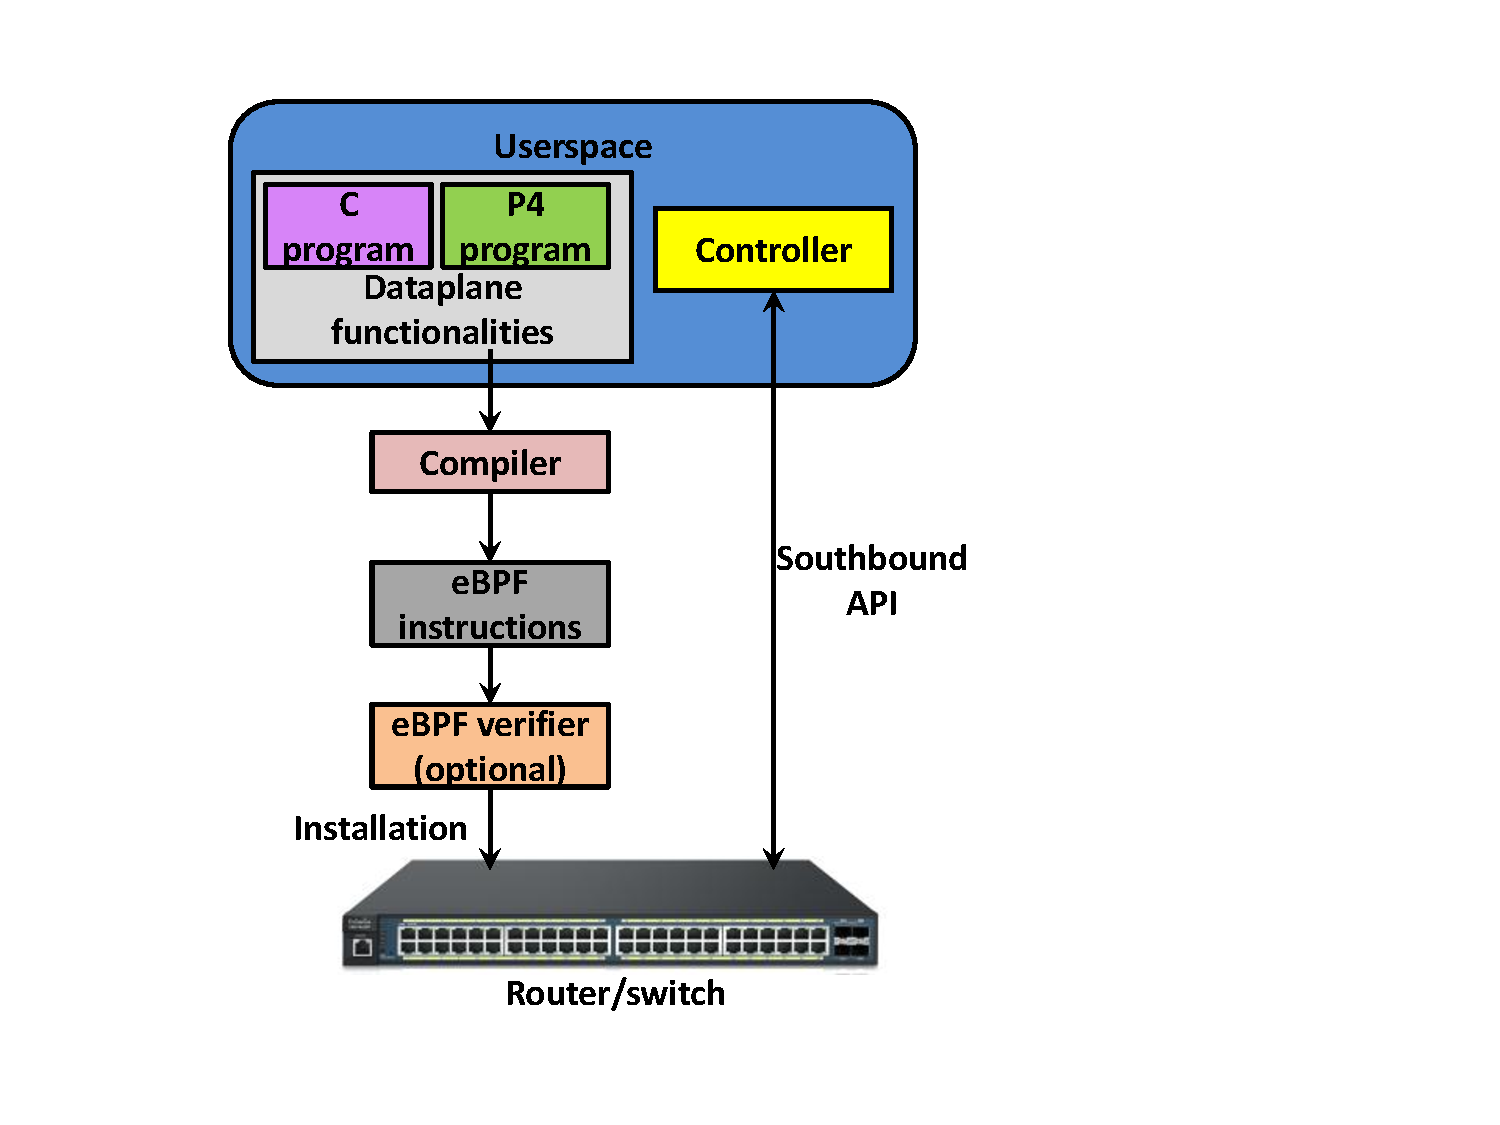
\includegraphics[width=.8\linewidth]{figures/Arquitetura2Crop.pdf}
% 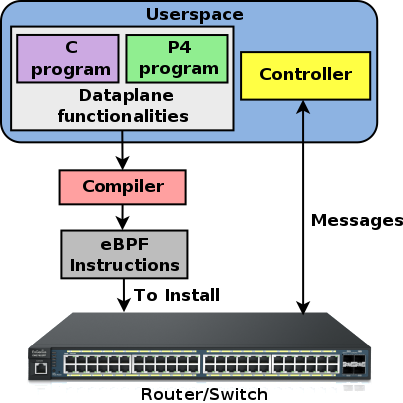
\includegraphics[width=.8\linewidth]{figures/03_fig01.png}
%  \caption{Architecture overview.}
%  \label{fig:03architecture}
%  \end{figure}

%Figure~\ref{fig:03architecture} provides an overview of the architecture.
The \system architecture has a logically centralized controller that communicates through a socket with the network elements (\eg routers, switches). 
Between the controller and the network elements, there is a southbound API that allows the controller to send platform-independent programs.

The controller can install programs in the data plane of the network elements at run time without network interruption (zero downtime).
The advantage of this approach is that the parser, matching, and actions can be modified at runtime.

%\subsection{Dataplane}

When designing the data plane, it should consider performance and how generic it is. It must be fast to be able to process the packets, presenting good network performance. Moreover,
the set of instructions must be generic to allow the implementation of various functionalities.

Our system has a generic packet processor, with no pre-established behavior.
The behavior of the device is defined by the set of instructions that accesses the packet headers, payload, and does the parser, matching, and actions at runtime.
The system uses the eBPF packet processor.

\subsection{eBPF}

%cBPF
Berkeley Packet Filter (BPF)\cite{McCanne:1993:BPF:1267303.1267305}, now referred as classic BPF (cBPF), is a "virtual machine" (called "pseudo-machine" originally) with a well-defined instruction set, which works as a low-level bytecode, conceptually similar to Java Virtual Machine (JVM) bytecode. It is used for packet filtering. Libpcap is an example of a library that uses BPF and is present at tcpdump and wireshark tools.



%eBPF
eBPF (extended BFP) is an improvement of BPF in which the architecture has been expanded from 32 to 64 bits, increased the number of write registers from 2 to 10, and added support for table operations and function calls~\cite{eBPF}.
Whereas BPF has only forward jumps, eBPF can have backwards and forwards jumps.
The Linux kernel, since version 3.18, allows userspace programs to install eBPF programs into the kernel. 
EBPF allows designing architectures independent of platforms or protocols.
No prior knowledge of the protocol or packet structure is required. 
To parse a packet, it is loaded into the eBPF data memory. The execution of the eBPF instructions moves the packet fields into registers and makes the necessary comparisons.

\begin{comment}
\begin{figure*}[ht]
\centering
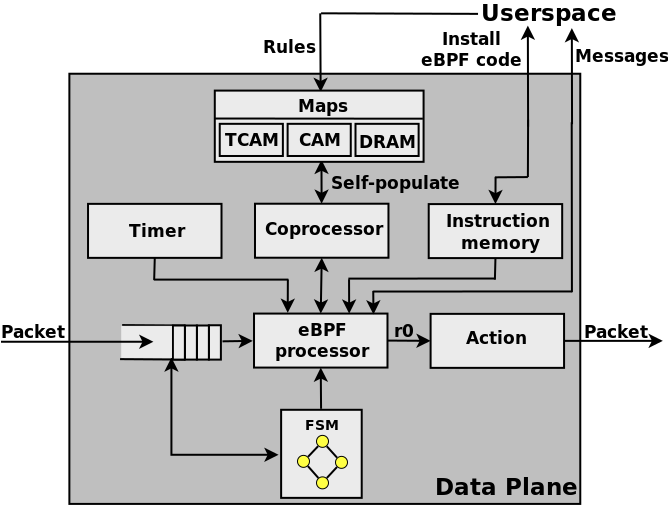
\includegraphics[width=.8\textwidth]{figures/06_fig01.png}
\caption{\system datapath implemented in NetFPGA SUME.}
\label{fig:06_fig01}
\end{figure*}
\end{comment}

%expressiveness
eBPF provides more expressiveness than OpenFlow.
OpenFlow matching structure has some limitations.
It is unable to do inequality, complement (not operation), or range matching~\cite{Jouet2015OpenFlow}. 
For instance, it can not do logical operations such as $\geq$ or $<$, which are needed for range expressions. 
If it needs a negation rule, for example, a match on a flow that is not on destination port 80 (web traffic), it needs to create rules for the other complement values. 
On the other hand, eBPF can express all these cases.
Moreover, OpenFlow switch can not extract Time-To-Live (TTL) or TCP Sequence Number fields, which are important to detect expiring packets and TCP migration, respectively. 
The OpenFlow solution to extract fields that are not part of the OpenFlow standard is to do it at the OpenFlow controller. 
On the other hand, an eBPF program containing only 6 instructions for each field can extract them.

%Top-of-Rack switches allows for approximately ~2000 OpenFlow flow entries.


%Table
In the software implementation of eBPF in the Linux Kernel, it can register a set of functions to handle maps, which is a < key; value > data structure. 
The most important functions are: create, lookup, update, and delete.
The eBPF program can invoke these functions executing the eBPF call instruction.
The types of maps include arrays, hashmaps, hashmaps with Least Recently Used (LRU) replacement policy, and, as of version 4.11, longest-prefix match (LPM) using trie.
These maps allow eBPF programs to keep state between packet arrivals.
In classic switches, layer 2 switch uses a hashmap lookup map to map the port associated with a MAC address.
IP routing maps the port associated to the destination IP with the LPM map.
Maps are important to store states.
In our hardware implementation, our design choice is to use hardware modules. The maps are content-addressable memory (CAM) for exact-matching, ternary content-addressable memory (TCAM) for LPM, and Dynamic Random Access Memory (DRAM) for arrays.


In this work, we propose to use the eBPF instruction set to parse, match, and define actions on the data plane.

\subsection{High-Level Languages}


High-level languages can be used to write code to the data plane and compile it into the eBPF instruction set. A subset of C already exists, which excludes some external libraries, system calls, and pointer arithmetic while providing functions for defining and manipulating tables. The LLVM 3.9 compiler has a backend for the eBPF platform, allowing programming in this subset of C and generating executable code in eBPF format.

It is also possible to generate eBPF instructions through specific domain languages, such as P4~\cite{Bosshart:2014:P4}.
There are efforts of the open source Iovisor project~\cite{IOvisor} and from VMware~\cite{p4c-xdp2018} that have already implemented a compiler from P4 to eBPF~\cite{P42EBPF2015}.

% \begin{figure}[htb]
% \centering
% %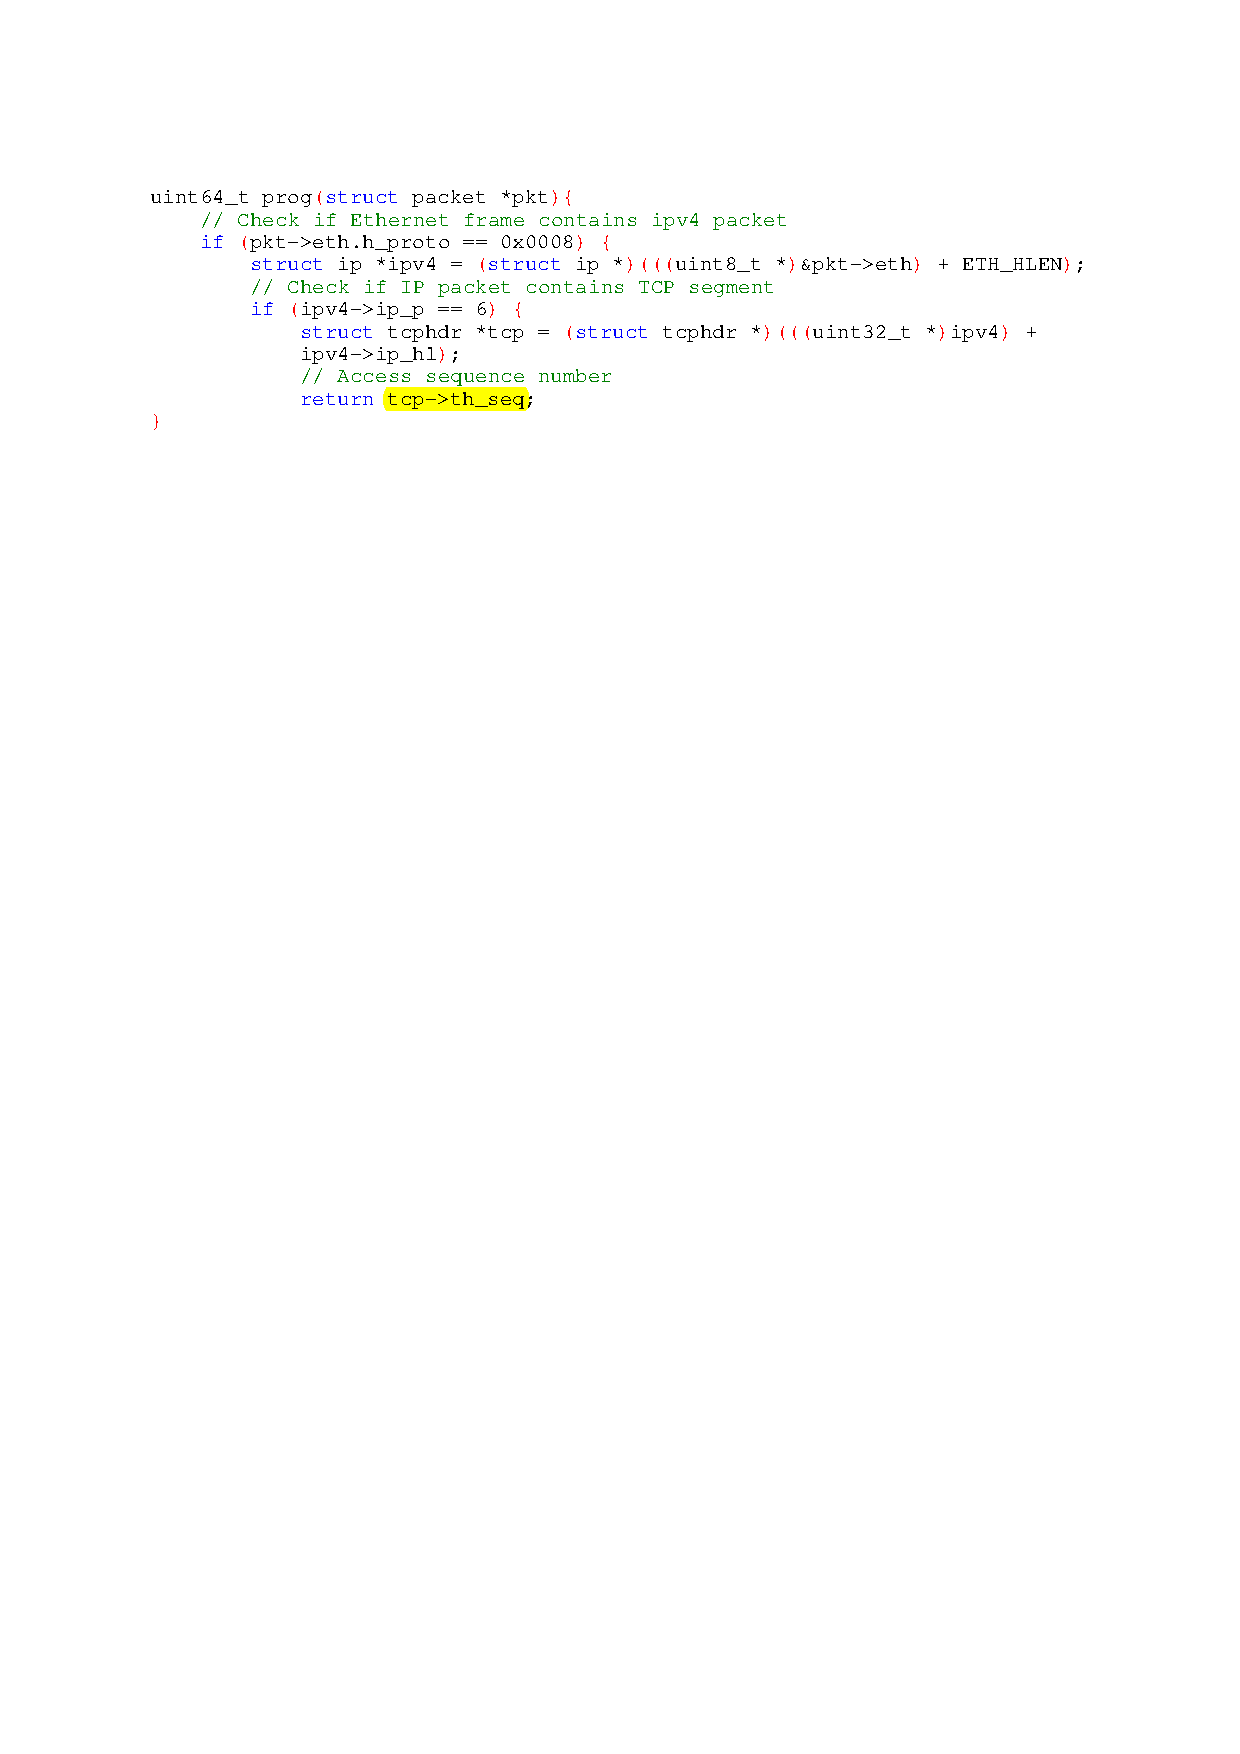
\includegraphics[width=1.\linewidth]{figures/sequenceNumber.pdf}
% 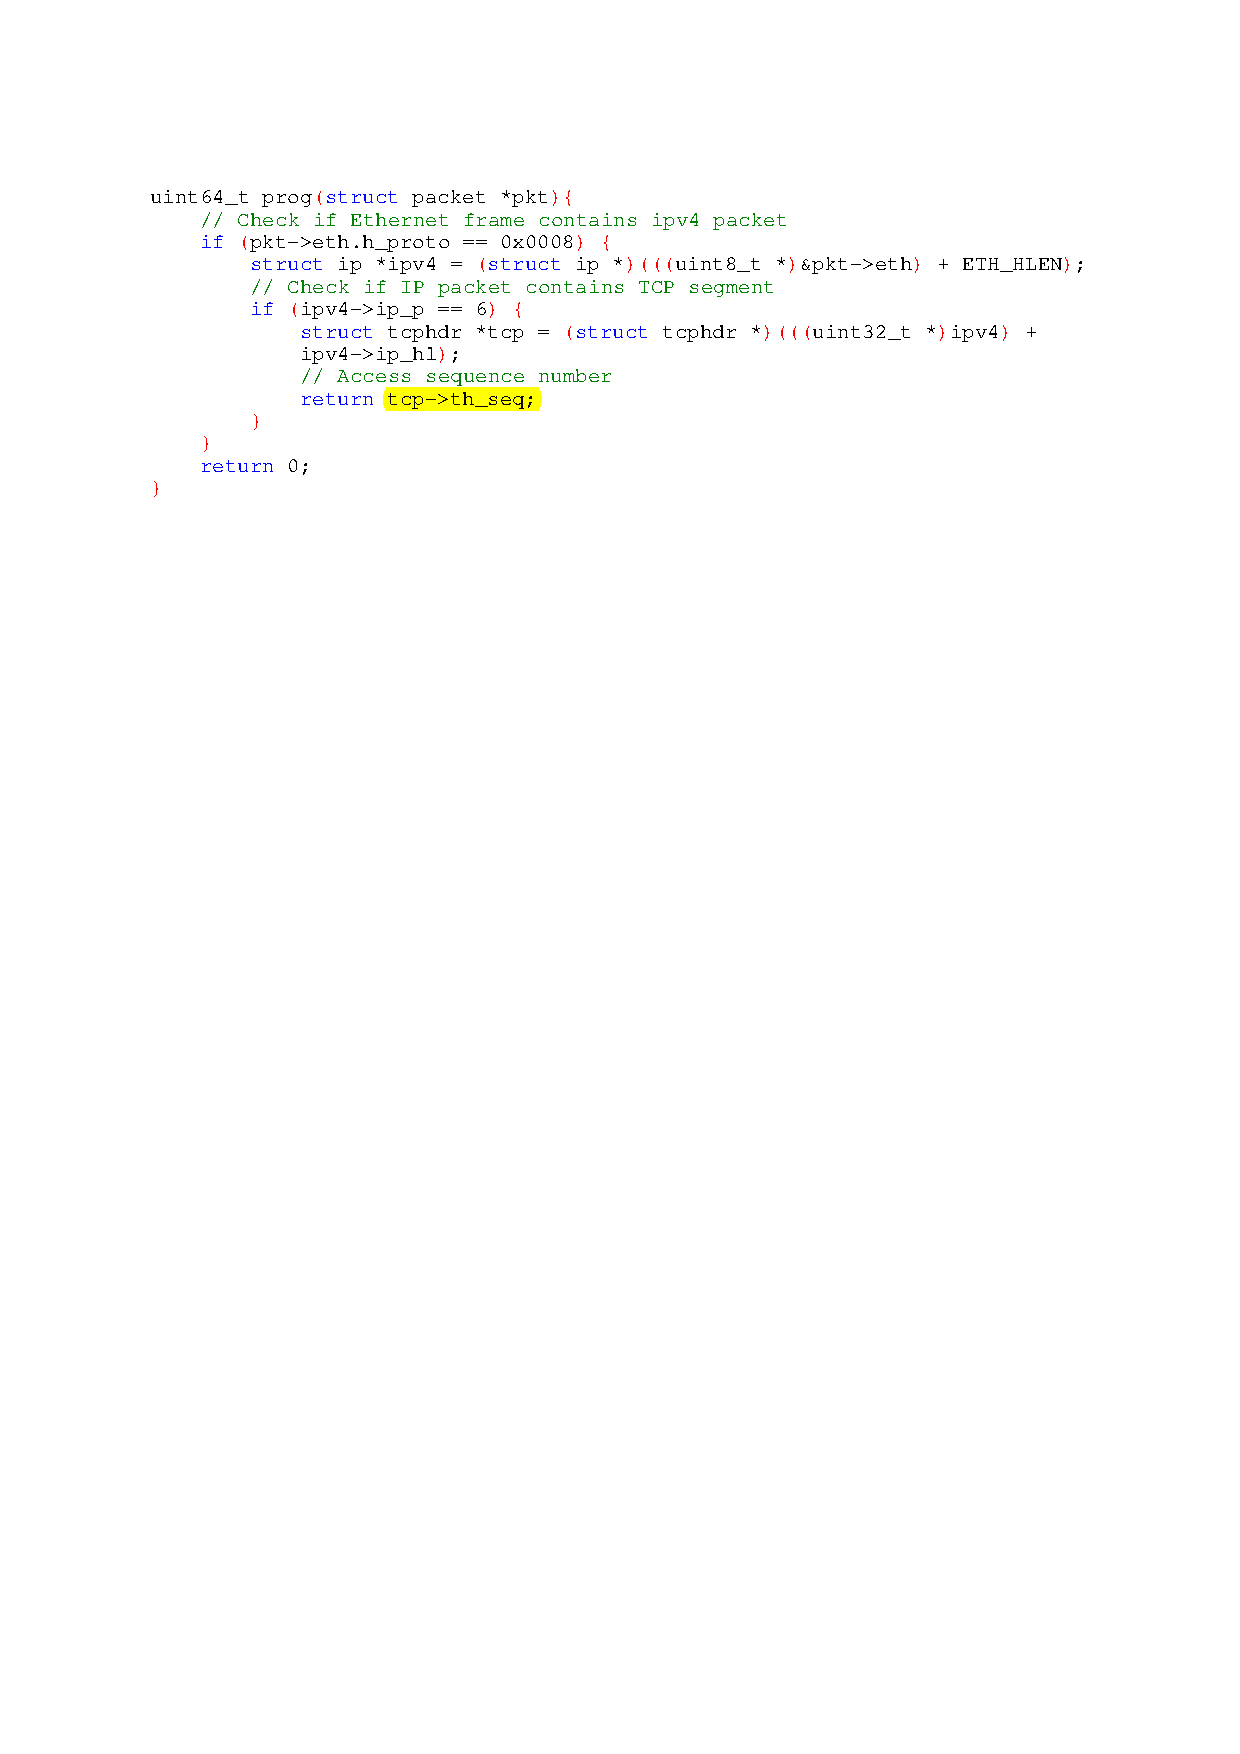
\includegraphics[width=1.\linewidth]{figures/seqnum.pdf}
% \caption{Example of a C program that accesses the TCP sequence number. This is not possible at the OpenFlow switch.}
% \label{fig:seqnum}
% \end{figure}

% Figure~\ref{fig:seqnum} illustrates an example of a field that can not be extracted at the OpenFlow switch but can be executed by eBPFlow: to analyze the TCP segment and access the sequence number.
% The code example, written in the subset of C, verifies that if it is an Ethernet frame that has an IP packet and contains a TCP segment. It then accesses the value of the TCP sequence number field. Dysco~\cite{Zave:2017:DSC:3098822.3098827} is an example of a system that provides a session protocol that requires the TCP sequence number.

% An important detail is that the LLVM compiler generates an executable in the executable and link format (ELF). This format has multiple segments for code execution. For our application, only the eBPF instruction set is required. The objdump tool allow to extract only the .text segment that has the instruction set. The controller installs this segment into the switch, which will execute these instructions.


% \begin{figure}[htb]
% \centering
% \includegraphics[width=.3\textwidth]{imagens/04_fig02.png}
% \caption{Diagrama de instalação das instruções eBPF no Switch/Roteador.}
% \label{fig:04_fig02}
% \end{figure}

%\subsection{Acyclic Control Flow Graph}
\subsection{eBPF verifier}
\label{sec:verifier}

%verifier
%There exits a verifier for programs with eBPF instructions.
The Linux kernel implementation provides an implementation of an eBPF verifier.
The verifier lets check the validity, security, and performance of eBPF programs.
If desired, the verifier allows eBPF programs with only bound-loops to enable static analysis.
The eBPF verifier checks whether a program terminates, whether the memory accesses are in the range of memory space, and the greatest depth of the execution path (critical-path).
This critical-path can provide an upper-bound on the execution time.
The verifier enables to provide eBPF kernel-safe code execution.
In eBPFlow, the verifier can be used after the code has been compiled and before loading it into the data plane.

% \begin{figure}[htb]
% \centering
% %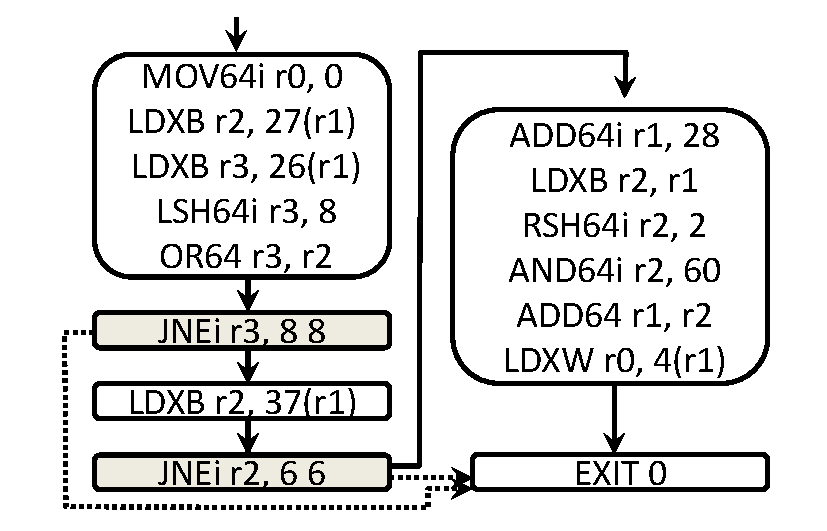
\includegraphics[width=.8\linewidth]{figures/eBPF_Acyclic_Control_Flow_Graph-_SeqNum3.pdf}
% 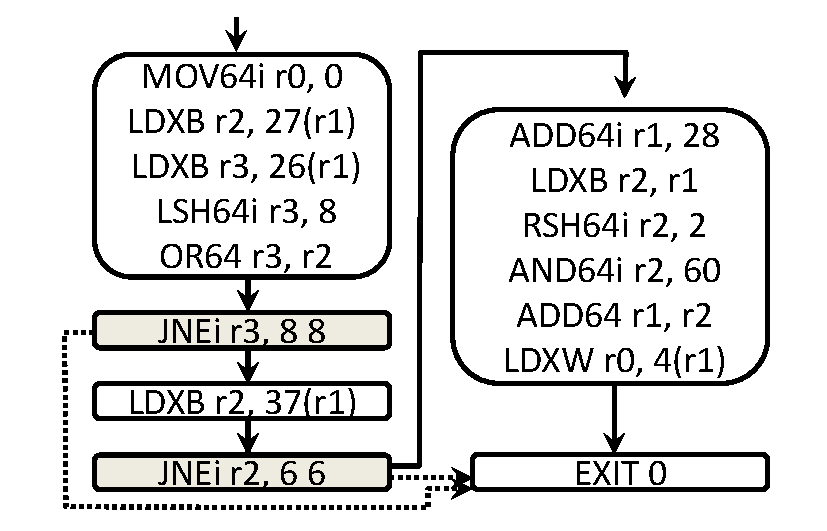
\includegraphics[width=.8\linewidth]{figures/eBPFACFG.pdf}
% \caption{eBPF Acyclic Control Flow Graph for the TCP sequence number example.}
% \label{fig:acfg}
% \end{figure}

% If the eBPF program has no backwards jump or just bound-loops (so loop unrolling can be applied), then the eBPF program can be synthesized into a directed Acyclic Control Flow Graph (ACFG). 
% Figure~\ref{fig:acfg} shows the ACFG to extract the TCP sequence number.% example presented in Figure~\ref{fig:seqnum}. 
% Each ACFG node contains one or more eBPF instructions. Instruction ending with the letter i indicates that the instruction uses an immediate value.

% The conditional jump nodes are the nodes that contain two output lines and light gray background.
% Solid line indicates the next ACFG node. Dotted line indicates a jump to another ACFG node.
% In our example, the conditional jump nodes contain the jump not equal (jnei) instruction.
% The last number of the jnei instruction indicates how many instructions to jump when the condition is valid.

% To better understand the eBPF program, let us explain that register r1 starts with a pointer to the packet and metadata (which we explain in Section~\ref{sec:metadata}) stored in the data memory and register r0 stores the return value.

% In the first node, load byte instructions extract the bytes 26 and 27 from the data memory.
% Given that the metadata has 16 bytes, this represents bytes 10 and 11 of the packet (counting from 0), which is the Ethernet type field. Then, a byte swap is done to set the endiness. 
% First jump instruction compares if the Ethernet type is 0x0800. Next, the IP protocol field is extracted from the IPv4 packet and checks if it is the TCP protocol (value 6). Finally, the TCP sequence number is extracted and placed in the return register (r0). The last instruction tells that the code terminates.
% ACFG is useful to determine the worst-case execution time.




%After presenting this example, we can better contextualize the general idea presented in  Figure~\ref{fig:03architecture}. In this scenario, 
The network manager writes a program in C or P4 language, and then compiles to eBPF. The eBPF program might be checked before installation with the eBPF verifier. The eBPF program is then installed on the device through the controller.

%O roteador executa essas instruções para cada pacote recebido, permitindo um plano de dados com análise, casamento e ações dinâmicas.

\subsection{Decoupling state from code}
%\subsection{Self-Populate}
\label{sec:selfpopulate}

eBPF enables to decouple code and state.
States are stored using maps.
The code is used to parse the packet.
For a matching, the code executes logical expressions and calls maps to query, for example, the next hop given the destination IP.
For actions, the code can modify the packet and indicates to where the packet should be forwarded.

% Given this decoupling, the eBPFlow can self-populate the tables. The eBPF instruction can call the maps functions to insert, delete, or update the tables. This is not possible with current P4 or OpenFlow standard where
% the controller is responsible for making
% all the forwarding decision, resulting in additional 
% network traffic, latency, and controller overload.
% Moreover, if desired, the controller can query the content of the tables anytime, 
% %or be notified when a table entry is  modified, 
%  thus, still having the knowledge of the entire network.


\subsection{Southbound API}
\label{sec:southboundAPI}

\begin{table}[htp]
\centering
\caption{Messages exchange between controller and network element.}
\label{tab:06_mes}
\resizebox{\linewidth}{!}{%
\begin{tabular}{|c|c|}
\hline
\textbf{Type of message} &  \textbf{Description}                                    \\ \hline
Hi                        &  Establish communication \\
%                          &  communication                                                                                                   \\ \hline
\hline
Install                  &  Install  eBPF\\
                         &  instruction on the device                                                                                       \\ \hline
%Notificação               & roteador $\rightarrow$  controlador                 & \begin{tabular}[c]{@{}c@{}}Roteador envia os dados lidos dos \\ registradores do hardware \\ para controlador\end{tabular} \\ \hline
\begin{tabular}[c]{@{}c@{}}Table \\ command\end{tabular}  & \begin{tabular}[c]{@{}c@{}}Controller send command\\ (update, delete, lookup, list) to device\end{tabular}               
\\ \hline
Packet In/Out                  &  Sends a packet to/from\\
                               & device from/to controller                                                                                       
\\ \hline

\end{tabular}}
\end{table}

The controller and device communicate via socket. After establishing the communication, both controller and network element can exchange messages with specific information. Table~\ref{tab:06_mes} displays the supported messages between controller and network element.

The first message sent after the communication is established is the "Hi" message. 
This message is sent to verify that the controller is connected to the network element and to obtain its datapath identification number. 
The message "Install" contains the eBPF instructions that will be installed in the instruction memory of the eBPF processor. 
The message "Table" contains commands for the tables in the device. It can update, delete, lookup, or list the content of the table. This is similar to OpenFlow when installing or removing a rule.
Packet\_in and Packet\_out messages are similar to OpenFlow. The device can ask the controller to make the decision about the packet and the controller can return a modified packet.
% "Notify" and "list tables" messages are used to capture information processed in the hardware, for example, the number of packets trafficked.



\section{Switch Design}
\label{sec:design}

\begin{figure}[!htbp]
\centering
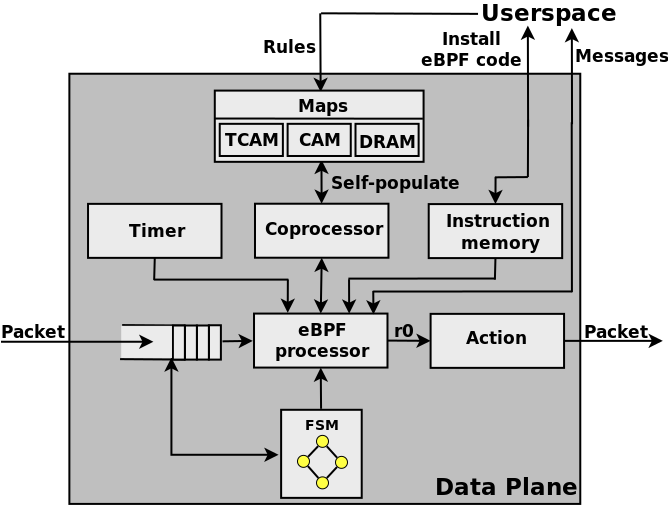
\includegraphics[width=1.\linewidth]{figures/06_fig01.png}
\caption{Switch datapath design and implementation on NetFPGA SUME.}
\label{fig:06_fig01}
\end{figure}

Figure~\ref{fig:06_fig01} gives an overview of the switch design and implementation on the NetFPGA SUME~\cite{SUME2014} platform. 
Each box represents a module.
The switch design is represented by the orange modules and Tables module.
The gray modules are the hardware modules that belong to the standard NetFPGA library and are described in Section~\ref{sec:implementation}.


\subsection{Data plane}

The switch extends the NetFPGA datapath with four new hardware modules (orange): instruction memory, eBPF processor, coprocessor, and action packet. There is also a modification to the Finite State Machine (FSM) of Output Port Lookup module. The eBPF instructions generated from the user-created C and P4 codes are stored in the instruction memory. These instructions define the behavior of the data plane. The eBPF processor is responsible for performing the parse, matching, and actions using instructions stored in the instruction memory. In addition, the processor communicates with the control plane through a socket. The coprocessor handles requests to access the tables. The action module in the packet only forwards or discards the packet according to the value stored in eBPF register r0 after processing the eBPF instructions. % Further details on the implementation of the data plan are presented in the \ ac {[ref]} section.

\subsection{Metadata}
\label{sec:metadata}

\begin{figure}[ht]
\centering
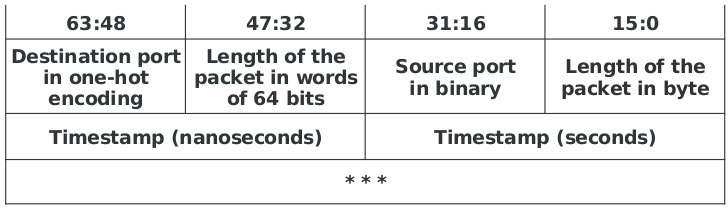
\includegraphics[width=1.\linewidth]{figures/06_fig03.png}
\caption{Metadata: Information retrieved from the input queue about the packet that is stored in the data memory of the eBPF processor.}
\label{fig:06_fig03}
\end{figure}

% \begin{table}[ht]
% \centering
% \caption{Metadata: Information retrieved from the input queue about the packet and stored in the data memory of the eBPF processor.}
% \begin{adjustbox}{max width=.8\textwidth}
% \label{tab:metadata}
% \begin{tabular}{|c|c|c|c|}
% \hline
% 63:48 & 47:32 & 31:16 & 15:0 \\
% \hline
% \begin{tabular}[c]{@{}c@{}}Destination \\port in one-hot\\encoding \end{tabular} &
% \begin{tabular}[c]{@{}c@{}}Length of the\\packet in\\words of 64 bits\end{tabular} &
% \begin{tabular}[c]{@{}c@{}}Source port\\ in binary\end{tabular} &
% \begin{tabular}[c]{@{}c@{}}Length of \\the packet \\in bytes\end{tabular} \\
% \hline
% \multicolumn{2}{|c|}{\begin{tabular}[c]{@{}c@{}}Timestamp (nanoseconds)\end{tabular}} &
% \multicolumn{2}{|c|}{\begin{tabular}[c]{@{}c@{}}Timestamp (seconds)\end{tabular}} \\
% \hline
% \end{tabular}
% \end{adjustbox}
% \end{table}


The data plane receives the packet through the input interface and stores the packet in the input queue with some additional information called metadata.
%Figure~\ref{fig:06_fig03} shows the stored structure.
Figure~\ref{fig:06_fig03} shows the metadata header. First line indicates the byte order and the other lines show the stored structure.
After the metadata is received, comes the Ethernet frame. Metadata header fields can also be used by the eBPF program, as well as, any other protocol field. The currently defined metadata are the destination port, packet size in multiples of 64-bit, source port, packet size in bytes, timestamp in nano seconds and seconds. The fields of packet size in multiples of 64-bit and bytes are included because the input queue module already provided this information.

\subsection{Actions}

\begin{table}[ht]
\centering
\caption{Action performed on the packets.}
\label{tab:action}
\begin{tabular}{|c|c|c|}
\hline
\textbf{Action}   & \multicolumn{1}{c|}{\textbf{Code}} & \textbf{Description} \\ \hline
\begin{tabular}[c]{@{}c@{}}Forwarding\end{tabular}  & 0 - 0xFFEF & Forwards packet. \\ \hline
Controller     & \begin{tabular}[c]{@{}c@{}} 0xFFF3\end{tabular}                           & Send packet to the controller. \\ \hline
\begin{tabular}[c]{@{}c@{}}Drop \end{tabular}  & 0xFFF0 & Drop packet. \\ \hline
\begin{tabular}[c]{@{}c@{}}Flood \end{tabular} & \multicolumn{1}{c|}{0xFFFF}  & \begin{tabular}[c]{@{}c@{}}Send packet to all ports\\ except for input port.\end{tabular} \\ \hline
\end{tabular}
\end{table}


The return value of the eBPF processor, which is stored in register r0, is used to determine which action should be performed with the packet. Table~\ref{tab:action} describes the return values of eBPF and their respective actions. After eBPF finishes its computation, the packet can be: forwarded to the exit port; forwarded to the controller; discarded; flooded to all ports with the exception of the input port.

%The NetFPGA hardware consists of four Ethernet ports. Each port contains one MAC and one CPU queues (Figure~\ref{fig:06_fig01}) where the packet can be routed. The coding values of the respective actions are based on the one-hot encoding of the queues.

eBPFlow enables other dynamic actions such as modifying the packet header, adding or removing fields.
Unlike RMT~\cite{bosshart2013forwarding}, eBPFlow can also modify the packet payload.
Since the packet is stored in the data memory, a store instruction modifies the packet. The packet content can also be used for arithmetic and logical operations, for example, decrementing TTL or recomputing checksum.


\section{Implementation}
\label{sec:implementation}

In this section, we describe the implementation details of \system.
The implementation consists of two components: data plane and user space tools. 
The data plane was implemented in the NetFPGA SUME platform~\cite{SUME2014}.
The user space tools are composed of a controller responsible for defining how the data plane will forward the packets, and software to configure the data plane features, according to the user-created C and P4 programs.


\subsection{Hardware Instance}

FPGA (Field Programmable Gate Array) enables to build hardware logic system.
%In this work, eBPFlow was implemented in NetFPGA SUME platform. 
The NetFPGA SUME hardware has four SFP+ transceivers that support 10 Gbps Ethernet ports.
It connects to a motherboard though an PCIe Gen 3 x8 adapter.
It contains a Xilinx Vertex-7 690T FPGA~\cite{Virtex7},
which has approximately 693,120 logic cells, a 27 MiB SRAM and 5 ns (200 MHz) clock cycle.
%\marcos{XXXX logic cells, a 4 KiB SRAM with $2^{19}$ lines and 8 ns (125 MHz)} clock cycle.

\textcolor{red}{The packets in the NetFPGA are processed in the form of 256-bit words and 128 bits control to identify the word type (data or metadata). Words are transmitted by the data signal and control. If control signal is zero, it means that the words of the packet are being transmitted, otherwise the words are from the metadata.}

%The packets in the NetFPGA are processed in the form of 64-bit words and 8-bit control to identify the word type (data or metadata). Words are transmitted by the data signal and the control by the ctrl signal. If the cntrl signal is zero, it means that the words of the packet are being transmitted, otherwise the words are from the metadata.

%The NetFPGA processes up to 64 bits of packet data per clock cycle (8 ns). Considering a packet size of 1,500 bytes and with that cycle, a packet takes approximately 2 $\mu{s}$ to be processed.

%The standard NetFPGA library provides the following modules: input arbiter, output port lookup and output queue. The input arbiter receives the packets from the network (via the MAC interface) or the PCI bus (via CPU) in the format of 64-bit words and stores them in internal queues of the module. Then, the words are taken from the queues using the round-robin algorithm, and it routes them to the output port lookup module.  The output port lookup module is responsible for defining which port the packet will be sent based on the packet properties, for example, an input port or destination address. The outgoing port of all incoming packets is configured in the metadata output port field. We implemented the device functionalities in the output port lookup module.

The standard NetFPGA library provides the following modules: input arbiter, output port lookup and output queue. The input arbiter receives the packets from the network (via the MAC interface) or the PCI bus (via CPU) in the format of 256-bit words and stores them in internal queues of the module. Then, the words are taken from the queues using the round-robin algorithm, and it routes them to the output port lookup module.  The output port lookup module is responsible for defining which port the packet will be sent based on the packet properties, for example, an input port or destination address. The outgoing port of all incoming packets is configured in the metadata output port field. We implemented the device functionalities in the output port lookup module.

\textcolor{red}{Table \ref{tab:eBPFresource} lists the logic and memory resource used by eBPFlow implementation on NetFPGA SUME.  We compared the resource used by eBPFlow with a reference switch.}      

\begin{table}[hbt]
\centering
\caption{NeFPGA's resource requirements for eBPFlow compared to reference switch.}
\label{tab:eBPFresource}
\begin{tabular}{|c|c|c|}
\hline
\textbf{Resource Type} & \textbf{Reference switch} & \textbf{eBPFlow} \\ \hline
\# Slice LUTs          & 49436 (11\%)              & 54085 (12.48\%)  \\ \hline
\# Block RAMs          & 194 (13\%)                & 200.50 (13.63\%) \\ \hline
\end{tabular}
\end{table}


\subsection{Finite State Machine of HW Controller}

The finite state machine (FSM) in the module output port lookup controls the whole operation of packet processing. It removes the packet from the internal queue of the module (forwarded by the input arbiter module), starts executing the eBPF instructions and forwards the packet to the next module (action packet) when the last instruction (\texttt{exit}) of eBPF is executed. The finite state machine is made up of eight states.

\subsection{eBPF Processor}

\begin{figure*}[hbt]
\centering
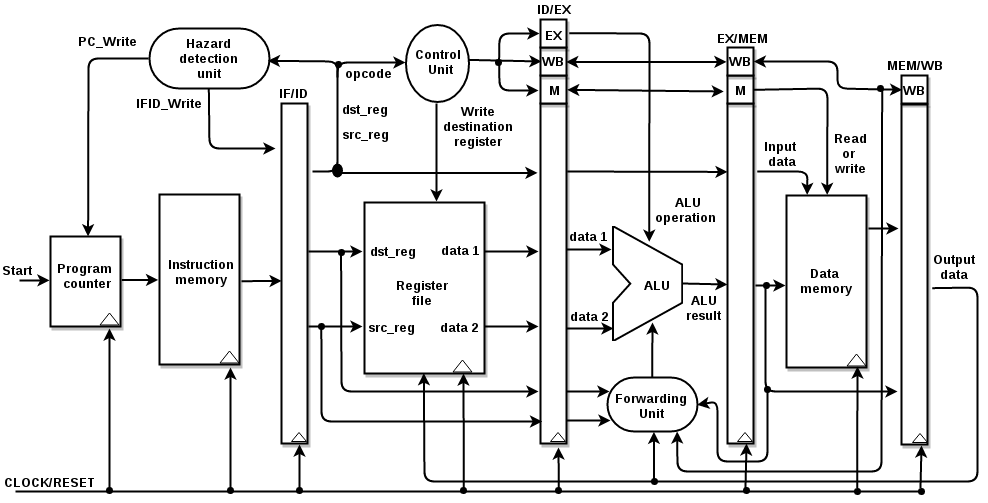
\includegraphics[width=.9\textwidth]{figures/06_fig02.png}
\caption{Control and Datapath of the eBPF processor.}
\label{fig:06_fig02}
\end{figure*}


The eBPF processor is responsible for performing the parse, matching, and actions according to the user-created user-generated C-code or P4-generated eBPF instructions. When starting the operation of the device, the user must load the eBPF instructions into the instruction memory to define  the behavior of the data plane.
% After the instructions have been loaded the switch starts processing the packets.

Figure~\ref{fig:06_fig02} presents the data and control path in register transfer level (RTL), containing five data functional units (program counter, instruction memory, register file, arithmetic logic unit (ALU), data memory) and three control units (hazard detection, forwarding, and control).

After the instruction is fetched from the memory instruction, it is divided into five parts: operation code, destination and source register address, offset, and immediate value. Each part of the instruction is sent to a specific unit. The control unit receives the operation code and forwards the control signals to the functional units, defining the behavior of each unit. For example, instructions in the ALU (arithmetic and logical unit) class do not use the data memory, so the read and write signals from the data memory are not activated.

The eBPF opcode is divided into seven classes: immediate load, load, immediate store, store, arithmetic and logical operations, jumps, 64-bit arithmetic and logical operations, and the other class is reserved for future use. The eBPF processor has 64-bit instruction, 32 bits for representing an immediate number (\texttt{imm}), 16 bits for offset, 4 bits for source register, 4 bits for destination register and, finally the 8-bit operation code (\texttt{opcode}). The opcode can be redivided depending on the instruction class. For load and store, the opcode has 3 most significant bits for memory access mode, 2 bits for word size and 3 bits for instruction class. For the jump instructions, logic and arithmetic, the 4 most significant bits specify what the operation is, 1 bit to specify whether the instruction is performed with the immediate value or with the source operand and, finally 3 bits less significant for the instruction class.

\begin{table}[ht]
\centering
\caption{Description of the eBPF register set.}
\label{tab:eBPFreg}
\begin{tabular}{|c|l|}
\hline
\textbf{Register} & \textbf{Description} \\
\hline \hline
R0 & return value from function, and exit value\\
\hline
R1 - R5 & arguments from eBPF program to function\\
\hline
R6 - R9 & callee saved registers that function preserve\\
\hline
R10 & read-only frame pointer to access stack\\
\hline
\end{tabular}
\end{table}

Read and write data operations in the registers are performed in the register file. 
In the read operation, the register file receives the addresses of the destination\/origin register and forwards the data referring to the ALU addresses. The write operation in the register file is performed after reading the data in the data memory or an ALU operation.
Table~\ref{tab:eBPFreg} describes the functionality of each eBPF register.

% Therefore, eBPF calling convention is defined as:
%
%    * R0	- return value from in-kernel function, and exit value for eBPF program
%    * R1 - R5	- arguments from eBPF program to in-kernel function
%    * R6 - R9	- callee saved registers that in-kernel function will preserve
%    * R10	- read-only frame pointer to access stack


The ALU of the eBPF processor is capable of performing arithmetic and logic operations based on the signal sent by the control. The ALU result can be forwarded as the data memory address or as the write data of the destination register in the register file.

The data memory has the functionality of storing metadata and packet words for the eBPF processor to perform the actions in the packet according to the eBPF instructions. There were two design options to implement the data memory: as register or at SRAM. Implementing the data memory as register has a delay of only 1 cycle in accessing it but consumes logical cells. The option of using SRAM does not consume logical cells but has a delay of 4 cycles. Since accessing the data memory is a critical operation, we opted to implement the data memory as a register file. The size of the data memory of the eBPF processor has a capacity of up to 256 words of 64 bits. With this capability, one metadata and one packet of up to 1,500 bytes can be stored. 
%We currently define the data memory with this capacity because of the little logical resource (53,000 logical cells) available in the NetFPGA SUME. 
The write operation is synchronous (only happens at clock edge) and the read operation is asynchronous.

The eBPF processor has a set of read and write instructions in the data memory with the following size types: 8 bits (byte (B)), 16 bits (half-word (H)), 32 bits (\ textit {word} (w)), and 64 bits (double word (DW)). In order to be able to read and write data of these size types, 
we add decoders and a control signal from the control unit to the decoders. The decoders perform the data mapping according to the control signal.
We also have to use the generate-for construct available by Xilinx tool. 
This construct does a loop unrolling before synthesizing the code and enables creating variable data size memory.

%We initially projected the eBPF processor for single-cycled datapath. Later, we extend it to a 5-stage pipeline:
We design the eBPF processor with a 5-stage pipeline: instruction fetch (IF), instruction decode (ID), execute (EXE), memory (MEM), and write back (WB).
IF stage gets instruction from memory and increments program counter (PC).
ID stage translates opcode into control signals and reads registers from the register file. EXE stage performs ALU operation, and computes jump/branch targets. MEM stage accesses data memory if needed. WB stage updates register file. 
This design follows the MIPS load-store pipeline architecture~\cite{Hennessy:2011:CAF:1999263}.
We add four pipelined registers (between the stages), the forwarding unit, and hazard unit. 

The forwarding unit is designed to solve the data hazards at ALU in a pipelined processor. The correct data at the output of the ALU is forwarded to the input of the ALU when data hazards are detected. These hazards are detected when the source register of the current instruction is the same as the destination register of the previous instruction.

The hazard detection unit is projected to solve data and control hazards. When data hazards occur, it needs to delay 1 cycle before forwarding.
Data hazard stalls 1 cycle when the destination register of the current instruction is the same as the source register of the coming instruction in ID stage. The control hazard happens when there is a jump/branch. In this case, the hazard detection unit discards instructions in IF and ID stages.
These units are implemented with logic gates to minimize latency.
Thus, we design an eBPF processor with a pipeline of 5 stages.


\subsection{Instruction Memory} 

%The eBPF instructions define the behavior of how the eBPF processor handles the packets. The instructions are inserted into the instruction memory via the NetFPGA register interface. Software registers were created to insert the eBPF instructions into the processor instruction memory. The instructions are received on the switch through messages sent by the controller. The instructions are then written to the software registers and forwarded to instruction memory via the hardware PCI bus.

%As a design decision, we have put the instruction memory outside of the eBPF processor in order to enable the connection of multiple processors in the future using a shared instruction memory. By increasing the number of eBPF processors in the datapath of the switch, more packets can be processed, contributing to the increase in the switch's throughput.

The eBPF instructions define the behavior of how the eBPF processor handles the packets. The instructions are inserted into the instruction memory via the NetFPGA register interface. Software registers were created to insert the eBPF instructions into the processor instruction memory. The instructions are received on the network element through messages sent by the controller. The instructions are then written to the software registers and forwarded to instruction memory via the hardware PCI bus.

\textcolor{black}{Instruction memory uses a double buffer system - DBS (Figure~\ref{fig:mem_db}) to provide zero downtime in the change of eBPF programs. This system is composed of two memories (M$_{1}$ and M$_{2}$). Both memories never assume the same state (writing or reading) at the same time. It means that while eBPF program is written to a memory, the eBPF processor reads the instructions of the other memory. DBS is initialized with eBPF instructions written on M$_{1}$, while M$_{2}$ remains idle. The system remains in the wait state until a new set of instructions will be received. After the instructions are written to M$_{1}$, the system will return to the standby state. When a new set of instructions is received, the memories change their states, which means that M$_{1}$ will no longer be written and will be read while M$_{2}$ will be written. If a new instruction set is received, these instructions are written in M$_{2}$, while the instructions previously written in M$_{1}$ are read and processed by the eBPF processor. This process can be repeated indefinitely.} 

\begin{figure}[ht]
\centering
\includegraphics[width=\linewidth]{figures/memory_db.png}
\caption{Instruction memory - Double Buffer System.}
\label{fig:mem_db}
\end{figure}

\textcolor{black}{As a design decision, we have put the instruction memory outside of the eBPF processor in order to enable the connection of multiple processors using a shared instruction memory. By increasing the number of eBPF processors, more packets can be processed, contributing to the increase in the throughput.}


\begin{comment}
%The eBPF instructions define the way in which the eBPF processor will process the packages. Instruction memory was implemented with a double buffer system in order to provide zero downtime in the prototype through important changes, such as sudden changes in the packet processing pattern. 

%The implementation of the double buffer memory started from the following design decision: the memories involved, M1 and M2, will never assume the same state (of writting or reading) at the same time. It means that while data is written to a memory, data is read from the other one and vice versa. 
%From this definition, we implemented an efficient management system that works as follows: the first memory to be written will always be M1, while M2 will remain idle. 
%The system remains in the wait state until a new set of instructions is received. Writing in M1 is initiated when a set of instructions is received. 
%Once all instructions are written to M1, the system will return to the standby state. When a new set of instructions is received, the memories will have their states changed, what means that M1 will no longer be written and will be read while M2 will be written. The new instruction set is then written in M2, while the instructions previously written in M1 are read and processed by the eBPF processor. This process is repeated indefinitely until the instruction sets are no longer received. In this case, the last written memory has its state maintained, that is, the state of write and read of the memories is only changed upon receipt of a new set of instructions. 
\end{comment}




\subsection{Maps}
\label{ssec:maps}

eBPF Linux kernel implementation allows for maps. Maps are a generic data structure that store different types of data in the form of key-value pairs. 
% Currently, the Linux Kernel allows for three different types of maps. Hash map applies a hash before inserting in the table. Array map accesses the table with an integer index. Program array map is used to store a program. eBPF programs can manipulate maps through specific kernel function calls, such as bpf\_map\_lookup\_elem().

In our design, we currently provide three types of maps: longest prefix matching (LPM), exact-match, and array map, which are provided in eBPFlow as hardware components. For LPM, we use the Ternary Content Addressable Memory (TCAM) module combined with the BRAM (Block RAM). TCAM is a specialized high-speed memory that does LPM searches very fast (1 cycle). TCAM uses three different inputs: 0, 1,  and "don't care". There is also the unmatchable (U) option provided by Xilinx design~\cite{xilinx_IP_2018} but we did not use it. Our TCAM module spends 16 cycles for a write operation and only 1 cycle for a read operation. For the exact-match, we use the Content Addressable Memory (CAM) module combined with the BRAM. For the array map, we use the DRAM memory.

The TCAM is implemented using Xilinx SRL16e primitives~\cite{xilinx_kylelocke2011}.
It is generated using Xilinx's IP core generator \textit{coregen}~\cite{xilinx_core_generator_2018}. The CAM is implemented using block RAM (BRAM) instead of SRL16e. This option enables to write on CAM using 2 cycles instead of 16 cycles.

There are three functions to manipulate the maps: update, delete, and lookup. The update operation updates an item into the map. If the item does not exist, it inserts the item. The delete operation removes the item with the given key. The lookup operation searches for the key and returns an item.
To manipulate these tables, the user can write C program and invoke the three functions through function calls.

\begin{figure}[ht]
\centering
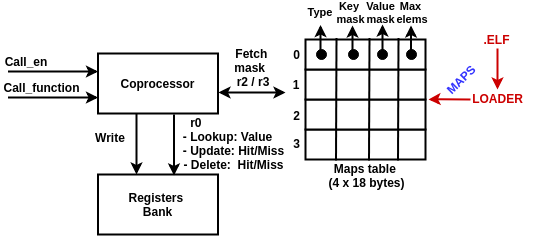
\includegraphics[width=1.\linewidth]{figures/coprocessor.png}
\caption{Coprocessor and Maps table.}
\label{fig:coproc}
\end{figure}

\textcolor{black}{
Since maps are generic data structures, allowing keys and values of multiple byte lengths, the coprocessor needs to know the actual size of the data being read/written to map memory. This information is stored in a \textit{maps table}, shown in Figure \ref{fig:coproc}, which holds metadata about each map declared in the current loaded program. This includes map type, key, value masks, and the maximum number of elements allowed in the map. 
%Our current implementation allows for maximum key and value sizes of 6 and 4 bytes, respectively.
The values are passed to the coprocessor by copy through registers R1-R4 on map calls. A lookup on the maps table is performed on every map operation to retrieve key and value masks, which are used in a bitwise-AND operation with the data to clean any unwanted bits. The map's type is also used by the coprocessor to switch to the proper memory unit (CAM or TCAM).
}

\subsection{Call instruction}

%eBPF allows invoking functions to access tables.
% The function calls are used to manipulate maps.
% In the Linux kernel, the software implementation of call functions is straightforward.
% There is a function pointer table. It registers the function call in the function pointer table.
% The call instruction is implemented as a function invocation thought the function pointer table.
% Parameters are passed through register 1 to 5. 

% The hardware call instruction implementation is different. It has to save the program counter (PC) value at the stack. It can pass parameters through registers or through the stack. Then, the processor executes an absolute jump to where the function instructions are located. 
eBPF allows invoking functions to access tables.
In our design, to manipulate maps, we opted to use the TCAM, CAM, and DRAM modules.
Thus, to manipulate tables, the function call inside the processor is replaced by a communication to the coprocessor hardware module. 
Thus, where there is call instruction, the processor communicates with the coprocessor module.
This module identifies what function (lookup, update, delete) was called though the call instruction immediate opcode parameter. 
Parameters are passed through register 1 to 4.
Register R1 indicates which hardware module to communicate (tables TCAM, CAM, DRAM, respectively).
Register R2 provides the key.
Register R3 stores the item.
Register R4 has the TCAM mask item.
Function return parameter is through register R0.
Since the call instruction requires register values, it can also suffers from hazard in the pipeline. The hazard unit has to stall to solve this issue.
Thus, for optimization, current call instruction is done through synchronous communication with coprocessor hardware modules since their functions are implemented in hardware.




\subsection{Synchronization}

\begin{figure}[ht]
\centering
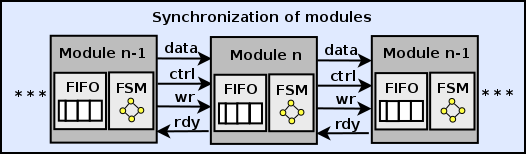
\includegraphics[width=\linewidth]{figures/06_fig04.png}
%\caption{Synchronization of the switch modules.}
\caption{Synchronization of the eBPFlow modules.}
\label{fig:06_fig04}
\end{figure}

\begin{comment}
The synchronization of the NetFPGA modules operates in a standardized way. Figure~\ref{fig:06_fig04} shows the synchronization of modules with their respective signals. The write (wr) and ready (rdy) signals control the communication between the modules. The wr signal informs when the previous module is ready to transmit (when it has content to transmit) and the rdy signal indicates that the next module is ready to receive. The transfer of data between modules only occurs if the two signals are active.

Each module contains an input queue and a finite state machine. The input queue is used to temporarily store the \textit{data} and \textit{ctrl} signal until the state machine module can remove the word from the queue. The state machine of each module has a specific behavior.
\end{comment}

\textcolor{black}{The synchronization of the NetFPGA modules operates of standardized way based on AXI-4 stream Xilinx protocol~\cite{XilinxAXI4}. Figure~\ref{fig:06_fig04} shows the 
modules' synchronism with their respective signals. TDATA represents the data stream. TUSER is out of band metadata. TKEEP marks qualified bytes (i.e byte enable). TLAST indicates end of packet/burst. The write (TVALID) and ready (TREADY) signals control the communication between the modules. The TVALID signal informs when the previous module is ready to transmit (when it has content to transmit) and the TREADY signal indicates that the next module is ready to receive. The transfer of data between modules only occurs if the two signals are active.} 

\textcolor{black}{Each module contains an input queue and a finite state machine. The input queue is used to temporarily store the TDATA, TUSER, TKEEP  and TLAST signals until the state machine module can remove the word from the queue. The state machine of each module has a specific behavior.}

\subsection{User space tools}

\color{black}{
The user space tools are composed of the controller and applications created at the user level.
The controller implements the Southbound API defined in Section~\ref{sec:southboundAPI}.
It was implemented in Python.
The controller opens a socket connection to the device to exchange the Southbound messages.

The applications to execute over the controller were also implemented in Python.
They open a connection to the controller and transmit the eBPF program, which was already compiled, as bytecodes.
These bytecodes are installed in the hardware by the controller at runtime.
In Section~\ref{sec:experiments}, we provide examples of applications.
}

\color{black}{
A set of tools were implemented as part of the eBPFlow infrastructure: an eBPF disassembler, a code loader (Section~\ref{ssec:loader}), a software emulator, and a CLI application to interact with the processor.

The emulator leveraged the uBPF\footnote{https://github.com/iovisor/ubpf} GitHub project and aims to replicate the processor's behavior in software. It enables code testing and debugging with well-known tools such as \textit{gdb}, enabling faster and easier bug detection and correction even before deploying the code to hardware.

In addition to these tools, many application examples were also created, as explained in Section~\ref{sec:experiments}.
}

\subsection{Loader}
\label{ssec:loader}
Loading code to the processor is done through the use of a \textit{loader}, specially designed for the eBPF processor. It serves two main purposes: modifying the code with processor specifics and interacting with its register interface.

At the beginning of every eBPF program, registers r1 and r10 need to be initialized with pointers to the packet, and to the top of the stack, respectively. Since these are specific to the runtime environment (here, the processor), such initialization is not part of the code generated by \textit{clang} compiler. Thus, when loading a program, the loader appends two instructions at the beginning of the instruction memory to correctly initialize those two registers with the proper addresses. 

To handle maps, the compiler adds map information to the eBPF ELF file as a relocation section, which needs to be processed before code execution. This job is also done by the \textit{loader}, which adjusts all map \textit{call} instructions with their corresponding map values according to the relocation table in the ELF file.

Finally, the \textit{loader} interacts with the processor register interface to load the list of instructions to the instruction memory and metadata about every map in the program to the maps table (Section \ref{ssec:maps}), after which the processor is ready to execute any incoming packets based on the loaded eBPF program. Through the register interface, the loader is also able to query status information about the processor, such as the value of r0, which instruction memory is being currently used and if the last load was successful or not.


\section{Results}
\label{sec:results}

\subsection{Validation of eBPF processor}

\begin{figure}[bth]
\centering
%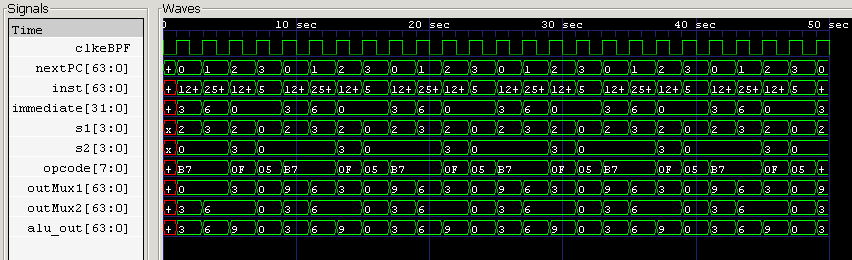
\includegraphics[width=1.\textwidth]{figures/07_fig02.png}
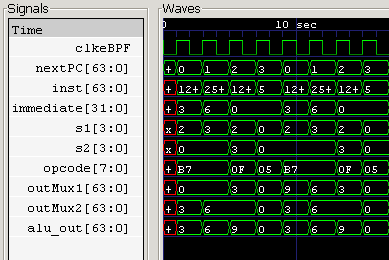
\includegraphics[width=1.\linewidth]{figures/07_fig02half.png}
\caption{eBPF processor waveform instruction tests.}
\label{fig:07_fig02}
\end{figure}


Firstly, for validation of the eBPF processor, we used the Altera Cyclone IV EP4CE115 platform. This FPGA has 114,480 logic cells, 50 MHz clock cycle and a set of memories (EEPROM, SRAM, Flash) with a storage capacity of 8 to 128 MB. We use the Altera platform with the aim of detecting and also correcting errors quickly before integrating the processor into the NetFPGA data path.


% \begin{figure}[H]
% \centering
% \includegraphics[width=1.\textwidth]{imagens/06_fig10.png}
% \caption{Forma de onda  processador eBPF.}
% \label{fig:06_fig10}
% \end{figure}




Figure~\ref{fig:07_fig02} presents the generated waveform of the execution of an assembly program containing the following instructions: mov64, add, and ja (jump absolute). The first instruction to execute is an immediate mov64. In this instruction, register r2 receives the immediate value 3. The second instruction is also an immediate mov64. The register r3 receives the value 6. In the third instruction, the sum operation between r2 and r3 is executed. Both operations use the register file to read and write to the respective registers. Register r2, at the end of the sum operation, has value 9 and stores it in the register file. The last instruction is a jump to the beginning of the code, the program counter goes to zero, initializing its operations. The last line in the Figure (alu\_out), represents the output of the ALU according to each instruction.


With the exception of the call instruction, as explained earlier, the eBPF processor has been synthesized and tested for all eBPF instructions on an Intel Altera platform. Then, the same processor was synthesized in Xilinx Vertex-II Pro 50 FPGA. Xilinx software synthesized all instructions except multiplication, division, and remainder instructions. In practice, these instructions are not widely used on a switch. In addition, these instructions with the power of 2 can be executed with the operations shift left, shift right, and logical operator and, respectively. We believe that a newer version of NetFPGA can accept the synthesis of these instructions. The project with the inclusion of these instructions, described in Verilog, is correctly synthesized in the Intel Altera FPGA development environment.

%Na figura~\ref{fig:06_fig11}

The eBPFlow was synthesized in the NetFPGA SUME and occupied 58\% of logical slice and 27\% of the register slice. The maximum frequency is 88.83 MHz (cycle of 11.25 ns).


\subsection{Experiments} 
\label{sec:experiments}

\begin{figure}[ht]
\centering
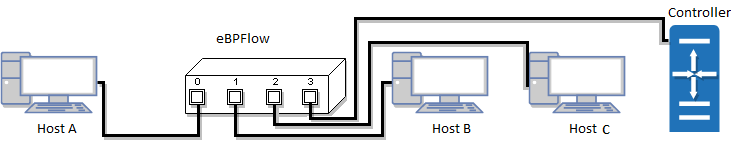
\includegraphics[width=1.\linewidth]{figures/07_fig03-3hosts.png}
\caption{Topology of the experiments.}
\label{fig:07_fig03}
\end{figure}

\begin{figure}[htb]
\centering
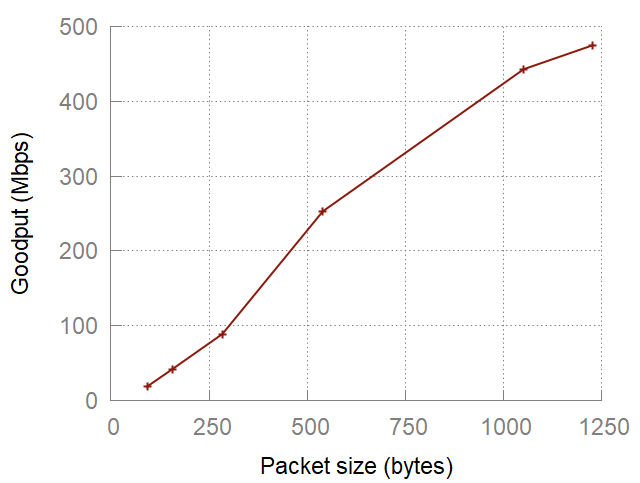
\includegraphics[width=1.\linewidth]{figures/goodputxbytes.png}
%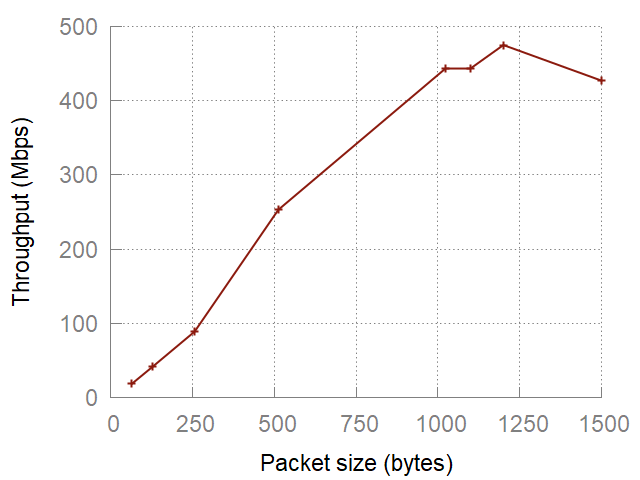
\includegraphics[width=1.\linewidth]{figures/throughputxbytes.png}
\caption{Goodput per packet size.}
\label{fig:07result}
\end{figure}

Figure~\ref{fig:07_fig03} presents the topology of the experiments. The NetFPGA has 4 ports. The switch interconnects three host computers and also connects to the controller.

We developed C language applications. The code is compiled with LLVM 3.9 for the eBPF big endian platform.
The LLVM compiler generates an executable in the executable and link format (ELF).
The objcopy tool extracts the instruction set from the .text segment of the elf file.
The controller installs this segment into eBPFlow.

The first application forwards frames from one interface to another. There is no learning involved, the output ports are hard-coded. Using the iperf tool, UDP connections are created between terminals A and B. Figure~\ref{fig:07result} shows the UDP goodput per packet size. This experiment evaluates what is the maximum obtained goodput.

The second example is an IPv4 router.
When eBPFlow receives a frame, it checks if the frame is an Ethernet frame and if it contains an IPv4 packet. It extracts the IPv4 destination and searches the TCAM for the output port.
The available actions are to forward the packet or drop it.
Figure~\ref{fig:IPv4routerresult} shows the goodput for UDP flow with packets of 1472 bytes.

\begin{figure}[htb]
\centering
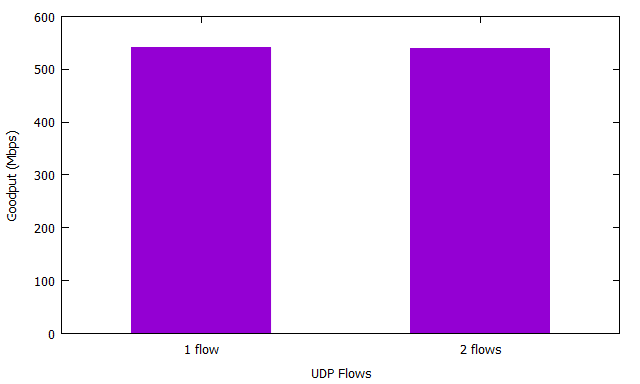
\includegraphics[width=1.\linewidth]{figures/ipv4goodput.png}
%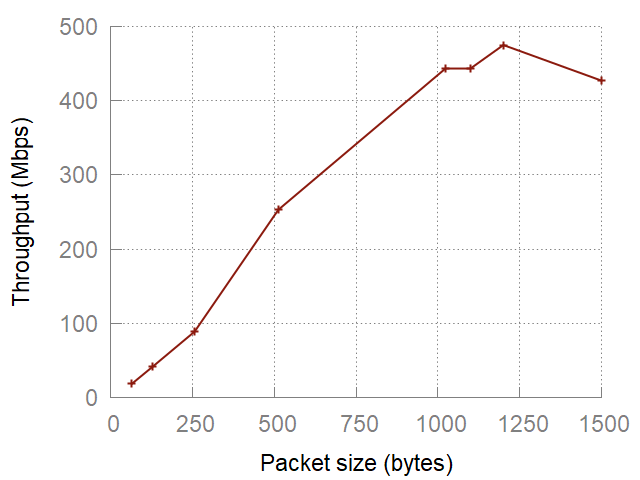
\includegraphics[width=1.\linewidth]{figures/throughputxbytes.png}
\caption{UDP Goodput for IPv4 router.}
\label{fig:IPv4routerresult}
\end{figure}

% \begin{table}[htb]
% \centering
% \begin{tabular}{|c|c|}
% \hline
% Number of Flows & Goodput (Mbps) \\
% \hline
% 1 & 541 $\pm$ 4.9 \\
% \hline
% 2 & 539 $\pm$ 13.99 \\
% \hline
% \end{tabular}
% \caption{UDP Goodput for IPv4 router.}
% \label{tab:IPv4routerresult}
% \end{table}


The third application is an L2 learning switch.
The advantage of a protocol-independent switch is that it only needs to parse the frame header fields for the protocols defined by the programmer. In this example, the parser only needs to parse Ethernet headers while protocol-dependent switch would process other frame or packet header fields. CAM (exact-match) lookup table stores the Ethernet MAC address and the input port. 
For each input frame, if the source address is unicast, the code can self-populate the lookup table by updating it.
This second advantage can reduce network traffic, latency, and CPU controller overhead.
Using the destination MAC, the output port is searched.
If there is an entry, then the packet is forwarded otherwise there are two options. It can be flooded or sent to the controller. In this experiment, we opted to flood.


The code is installed through the NetFPGA register interface.
The time to read or write one register in this interface is 500 us.
Each eBPF instruction (64 bits) utilizes two registers (32 bits).
To start the code installation, it requires 2 write operations.
Thus, the time to install a code is given by:\\
Time to install code $=$ (number of instructions+2) $* 500 us * 2.$ 

In the last experiment, eBPFlow starts as IPv4 router. During runtime, we install the learning switch. This experiment validates the system by showing that the switch executes these instructions for each received packet, allowing a data plane with dynamic parse, matching, and actions at run time with zero downtime.

\subsection{Power}

When idle, the NetFPGA consumes 16 W.
When eBPFlow is loaded, the power consumption is 22 W independent of the packet rate or what programming is running.
On the other hand, an idle CPU already consumes 85 W.
Thus, eBPFlow saves power in comparison to software packet processing.



\section{Discussion}
\label{sec:discussion}

% \subsection{Analysis}

% Here, we provide an analysis on the upper bound on the number of instructions that can be executed, given the eBPF processor clock and the interface speed.

% From Ethernet standard (IEEE 802.3)~\cite{EthernetStandard}, the preamble has 7 bytes and the start of frame delimiter (SFD) has 1 byte. The interframe gap (IFG) is composed of 12 bytes.
% So, for every frame of X bytes, the link transmits (X+20) bytes, or (X+20)*8 bits. Thus, the number of frames per second (\#fps) to be processed is equal the interface speed (bps) divided by (frame\_size(bytes)+20)*8.

% The time to process one frame is 1/\#fps.
% For a single stage processor (clocks per instruction (CPI) equals 1), the processor can execute clock (Hz) instructions.
% Suppose that the time to process a frame is spent only on the eBPF processor, the number of instructions that can be executed by a given interface speed and frame size is: clock(Hz)/\#fps.

% \begin{figure}[htb]
% \centering
% 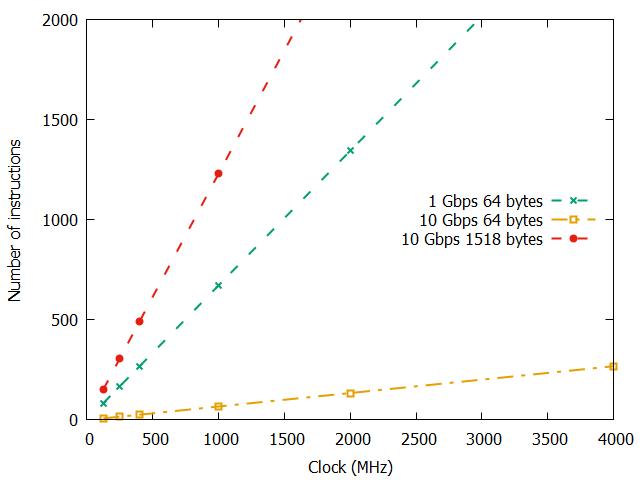
\includegraphics[width=1.\linewidth]{figures/numberInstructionsPerClock.png}
% \caption{Maximum number of instructions that can be processed given CPU clock (MHz),  interface speed (Gbps), and frame size (bytes).}
% \label{fig:instructionsPerClock}
% \end{figure}

% Figure~\ref{fig:instructionsPerClock} shows the upper bound of eBPF instructions that can be processed, given the eBPF processor clock in MHz, the interface speed in Gbps, and the frame size (bytes). The smaller is the frame size, the large is the number of frames to process. Thus, smaller frames require to be processed with fewer eBPF instructions. For 10 Gbps links, a frame size of 64 bytes, and 1 GHz clock, the maximum number of instructions is 67.
% Current CPU desktops operate at near 4 GHz, which results in an upper bound of 268 instructions.


\subsection{Limitations}

% Nao sei se coloca esse paragrafo.
%
% Currently implementation only support one table for each matching type (LPM, exact-matching, array). In practice, this is not harmful since usually only one LPM table is required (for IP matching). Moreover, exact-matching table can incorporate many tables, as long as items do not share the same key. But, ideally, eBPFlow should receive an ELF file containing the structure of the tables and map them to hardware or a compiler would map logical lookup tables to physical tables~\cite{Lavanya2015CompilingTable}.

% For a matching field that belongs to the OpenFlow standard, it might require only 1 flow rule and 1 TCAM lookup, while eBPFlow requires at least four instructions (one load of packet field, one load of the data value to be compared, one comparison and branch, one return value). But on the other hand, 

eBPFlow allows for logical expressions (not, and, or) and range comparison($>$,$<$). OpenFlow would require more rules and the number of rules (memory) is important in TCAM. 
% Moreover, as shown in Figure~\ref{fig:instructionsPerClock}, spending some eBPF instructions, for example 4, to parse a packet is acceptable.

% In current implement, the eBPF processor is a shared resource for all input queues.
% We plan, for future work, to place an eBPF processor for each input queue. 
% In this case, a NetFPGA with a larger number of cells is required.
% Our system has already been designed to integrate multiple eBPF processors. This is the reason that, in our design, the instruction memory is already in another module separated from the eBPF processor. 
% Instruction memory could be read in parallel by several eBPF processors simultaneously.

% Currently eBPFLow implementation on NetFPGA SUME provides \marcos{XXXXX} throughput (Figure~\ref{fig:07result}). 
%This is due to the limitations of NetFPGA 1G platform. 
% FPGAs are useful for prototyping and validating the hardware logic design~\cite{cofer2005rapid,sukhwani2017contutto}. 
% The logic design for FPGA shares the same initial flow and methodology as ASIC design~\cite{kuon07measuring,ASICDesignFlow2005}. 
% We leave eBPFlow over ASIC as future work.


\section{Related Work}
\label{sec:relatedWork}

%\begin{table*}[!htp]
\centering
\caption{Related Work Overview}
\begin{adjustbox}{max width=\textwidth}

\label{tab:05related_work}
\begin{tabular}{|c|c|c|c|c|c|c|c|}
\hline
\textbf{Related Work}                                                                                                                                         & \textbf{Description}                                                                                          & \textbf{Year} & \textbf{Language}                                                                       & \textbf{\begin{tabular}[c]{@{}c@{}}Hardware\\ or\\ Software\end{tabular}} & \textbf{Model}                                                                                 & %\textbf{\begin{tabular}[c]{@{}c@{}}Estudo de caso(s) \\ implementado(s)\end{tabular}}                                    
\textbf{\begin{tabular}[c]{@{}c@{}}Zero \\ Downtime\\ installation \end{tabular}}
& \textbf{\begin{tabular}[c]{@{}c@{}}Self\\Populate\\Tables \end{tabular}}
\\ \hline
\textbf{eBPFlow} & \begin{tabular}[c]{@{}c@{}}Arquitecture with \\ eBPF hardware\end{tabular} & 2018 & \begin{tabular}[c]{@{}c@{}} C or P4\\ for eBPF \end{tabular}  & Hardware & NetFPGA 1G                  & \checkmark & \checkmark
\\ \hline
\begin{tabular}[c]{@{}c@{}}P4FPGA\\ \cite{p4fpga}\end{tabular}                                                  & \begin{tabular}[c]{@{}c@{}}Implementation of P4 \\ in hardware\end{tabular}                                     & 2017         & \begin{tabular}[c]{@{}c@{}}P4 for \\ Verilog\end{tabular}                        & Hardware                                                                  & \begin{tabular}[c]{@{}c@{}}FPGA \\ Virtex 7 \\ XC7V690T\end{tabular}                  & %\begin{tabular}[c]{@{}c@{}}Encaminhamento L2/L3, \\ Paxos e protocolo \\ de dados de mercado\end{tabular}
&
\\ \hline
\begin{tabular}[c]{@{}c@{}}FlexPipe\\ \cite{FlexPipe2012}\end{tabular}                                & \begin{tabular}[c]{@{}c@{}}Reconfigurable \\match-action\end{tabular} & 2012         & \begin{tabular}[c]{@{}c@{}}Microcode \end{tabular}                        & Hardware                                                                  & FM6000                                                                                     & 
&
\\ \hline

\begin{tabular}[c]{@{}c@{}}dRMT\\ \cite{chole2017drmt}\end{tabular}                                & \begin{tabular}[c]{@{}c@{}}Reconfigurable \\ match-action\end{tabular} & 2017         & \begin{tabular}[c]{@{}c@{}}  P4 \end{tabular} & Hardware                                                                  & \begin{tabular}[c]{@{}c@{}} dRMT\\ hardware\end{tabular}   &         &
\\ \hline

\begin{tabular}[c]{@{}c@{}}POF\\ \cite{Song:2013:POF:2491185.2491190}\end{tabular}                                & \begin{tabular}[c]{@{}c@{}}Protocol \\ independent switch\end{tabular} & 2013         & \begin{tabular}[c]{@{}c@{}} flow \\instruction\\ set \end{tabular}   &  \begin{tabular}[c]{@{}c@{}} Hardware\\ and\\ Software\end{tabular}                                                                 &  Huawei  &          &
\\ \hline

\begin{tabular}[c]{@{}c@{}}BPFabric\\ \cite{Jouet:2017:BPFabric}\end{tabular}                       & \begin{tabular}[c]{@{}c@{}}Arquitecture with \\ eBPF support\end{tabular}                                     & 2017         & \begin{tabular}[c]{@{}c@{}} C or P4\\ for eBPF \end{tabular}          & Software                                                                  & Intel DPDK        & 
%\begin{tabular}[c]{@{}c@{}}L2 learning, \\ telemetria na rede e \\ detecção de anomalia\end{tabular}
\checkmark
& \checkmark
\\ \hline
%\begin{tabular}[c]{@{}c@{}}Workshop tutorial P4 \\ na NetFPGA \\ SIGCOOM \\ ~\cite{ACMSIGCOMM2017}\end{tabular}                                                      & \begin{tabular}[c]{@{}c@{}}Implementação P4 \\ em hardware\end{tabular}                                     & 2017         & \begin{tabular}[c]{@{}c@{}}P4 para \\ linguagem \\ descrição de \\ hardware\end{tabular} & Hardware                                                                  & \begin{tabular}[c]{@{}c@{}}NetFPGA \\ SUME - \\ FPGA \\ Xilinx \\ Virtex-7 \\ 690T\end{tabular} & \begin{tabular}[c]{@{}c@{}}Detecção heavy hitter, \\ monitoramento de rede, \\ packet fuzzer e tic-tac-toe\end{tabular}                                   \\ \hline
%\begin{tabular}[c]{@{}c@{}}P4 Compiler \& \\ Interpreter: \\ A Survey~\cite{stubbe2017p4}\end{tabular}                                                        & \begin{tabular}[c]{@{}c@{}}Visão geral dos \\ conceitos e softwares \\ da linguagem P4\end{tabular}         & 2017         & -                                                                                        & -                                                                         & -                                                                                               & -                                                                                                                                                         \\ \hline
%\begin{tabular}[c]{@{}c@{}}P4-to-VHDL: \\ Automatic \\ Generation of 100 Gbps \\ Packet Parsers \\ ~\cite{benacek2016p4}\end{tabular}                               & \begin{tabular}[c]{@{}c@{}}Implementação  gerador \\ analisador de pacotes\end{tabular}                     & 2016         & \begin{tabular}[c]{@{}c@{}}P4 para \\ VHDL\end{tabular}                                  & Hardware                                                                  & \begin{tabular}[c]{@{}c@{}}FPGA \\ Xilinx \\ Virtex-7 \\ XCVH580T\end{tabular}                  & \begin{tabular}[c]{@{}c@{}}Pilha de \\ protocolo \\ completa e \\ L2 simples\end{tabular}                                                                 \\ \hline
\begin{tabular}[c]{@{}c@{}}PISCES\\ \cite{Shahbaz:2016:Pisces}\end{tabular}                                & \begin{tabular}[c]{@{}c@{}}Switch \\ with P4 support\end{tabular} & 2016         & \begin{tabular}[c]{@{}c@{}}P4 for \\ binary code\end{tabular}                        & Software                                                                  & OpenvSwitch                                                                                     & %\begin{tabular}[c]{@{}c@{}}Análise Ethernet, \\ encapsulamento VLAN, \\ protocolos TCP/UDP\end{tabular}                                          
&
\\ \hline

%\begin{tabular}[c]{@{}c@{}}HyPer4: Using P4 to \\ Virtualize the \\ Programmable \\ Data Plane \\ ~\cite{hancock2016hyper4}\end{tabular}                               & \begin{tabular}[c]{@{}c@{}}Virtualização \\ programas P4\end{tabular}                                       & 2016         & -                                                                                        & Software                                                                  & -                                                                                               & \begin{tabular}[c]{@{}c@{}}Comutador \\ ethernet L2, \\ roteador IPv4, \\ proxy ARP e \\ firewall (tráfego \\ IPv4, TCP e UDP)\end{tabular}               \\ \hline
%\begin{tabular}[c]{@{}c@{}}High speed packet forwarding \\ compiled from protocol \\ independent data plane\\ specifications \\ ~\cite{laki2016high}\end{tabular} & \begin{tabular}[c]{@{}c@{}}Implementação \\ protótipo \\ compilador P4\end{tabular}                         & 2016         & \begin{tabular}[c]{@{}c@{}}P4 para \\ código C\end{tabular}                              & Software                                                                  & Intel DPDK                                                                                      & \begin{tabular}[c]{@{}c@{}}Encaminhamento \\ L2/L3  e  um \\ protocolo imaginário \\ na linguagem P4\end{tabular}                                         \\ \hline
%\begin{tabular}[c]{@{}c@{}}One Sketch to Rule Them \\ All: Rethinking \\ Network Flow \\ Monitoring with \\ UnivMon \\ ~\cite{liu2016one}\end{tabular}           & \begin{tabular}[c]{@{}c@{}}Framework de medição \\ baseada em scketches \\ com suporte a P4\end{tabular}    & 2016         & -                                                                                        & Software                                                                  & -                                                                                               & \begin{tabular}[c]{@{}c@{}}Detecção de \\ heavy hitter e DDoS, \\ troca de tráfego, \\ estimação de entropia e \\ detecção de iceberg global\end{tabular} \\ \hline
%\begin{tabular}[c]{@{}c@{}}P4 and \\ OpenvSwitch \\ ~\cite{P42014}\end{tabular}                                                                             & \begin{tabular}[c]{@{}c@{}}Integração P4 \\ com EBPF no \\ OpenvSwitch\end{tabular}                         & 2015         & \begin{tabular}[c]{@{}c@{}}P4 para \\ instruções eBPF\end{tabular}                       & Software                                                                  & OpenvSwitch                                                                                     & -                                                                                                                                                         \\ \hline
%\begin{tabular}[c]{@{}c@{}}DC.p4: Programming the \\ Forwarding Plane of \\ a Data-Center Switch \\ ~\cite{sivaraman2015dc}\end{tabular}                             & \begin{tabular}[c]{@{}c@{}}Estudo de caso P4 \\ em switches de \\ Data Centers\end{tabular}                 & 2015         & -                                                                                        & Software                                                                  & Mininet                                                                                         & -                                                                                                                                                         \\ \hline
\end{tabular}
\end{adjustbox}
\end{table*}


To the best of our knowledge, eBPFlow is the first packet processing hardware device that is Turing-Complete, enables the programming of stateful and stateless network functions, and can dynamically modify the parser, matching, and actions at zero downtime.
%and can also self-populate its tables.

%OpenFlow standard 
\textbf{OpenFlow standard}. The OpenFlow~\cite{McKeown:2008:OpenFlow} standard, although being the most adopted SDN architecture, has limitations. Its matching structure is unable to do inequality, complement (not operation), or range matching. 
%OpenFlow does not support self-populating the tables. It delegates the responsibility entirely to the controller.


% P4, C, Domino
%todo: C?
\textbf{High level domain specific languages.} The P4 programming language P4~\cite{Bosshart:2014:P4} adopts the match-action abstraction model. 
%does not have yet support for programs that self-populate the tables. It might be a possible future improvement, which is currently limiting the design of new data plane functionalities.
P4 language can be used to generate eBPF instructions using the compiler from P4 to eBPF~\cite{P42EBPF2015}. Domino~\cite{Sivaraman:2016:PTH:2934872.2934900} is a high-level language that can be compiled into Banzai, which is a low-level machine model designed for line-rate switches. 
Although P4 and Domino include small and fast registers to store state, they provide a restricted functionally for large range of stateful functions.

%- POF, NetASM
\textbf{Intermediate level domain specific languages.} Some works(~\cite{Song:2013:POF:2491185.2491190,Shahbaz:2015:NetASM,Sivaraman:2016:PTH:2934872.2934900}) define an intermediate instruction set to improve the data plane programmability.
Protocol Oblivious Forwarding (POF)~\cite{Song:2013:POF:2491185.2491190} from Huawei describes a protocol-independent programmable SDN switch. POF defines a generic flow instruction set (FIS) to search and extract keys from the header fields and also modifying packets and updating match tables. NetASM~\cite{Shahbaz:2015:NetASM} defines an instruction set with 23 instructions and provides an intermediate representation for programmable data planes. It can be used as the target language for virtual switches and line-rate switches. 

% DPDK, NetMap
\textbf{Packet I/O.}   Data Plane Development Kit (DPDK) framework~\cite{DPDK2018} is a set of packet I/O libraries that consumes CPU cores for fast packet processing. 
eXpress Data Path (XDP)~\cite{Hoiland-Jorgensen:2018:EDP:3281411.3281443} is a kernel hook for fast software packet processing, allowing to execute BFP programs inside the Linux kernel.
Following the same direction, NetMap~\cite{rizzo2012netmap} is an API that enhances access to network packets by user space applications.
%Those solutions are not transparent, thus requiring from the network programmer knowledge about the implementation details. 


% OvS, Pisces
\textbf{Software switches.} PISCES~\cite{Shahbaz:2016:Pisces} is a software switch based on OpenVSwitch (OVS)~\cite{Pfaff:2015:OpenVSwitch} that supports the high-level language P4. 
%P4 is used to define the prototype data plane. 
PISCES switch is a modified version of OVS with parsing, matching, and actions generated by the P4 compiler. 
PISCES can express conditionals (and) and relational tests ($>,<$) comparison of header fields.
%PISCES project is not designed to run on hardware.
%PISCES é voltado para processamento de pacotes em software para em centros de dados.
PISCES generated code must be recompiled for each modification in the P4 program. Click~\cite{kohler2000click} is a modular software router architecture that has been used in different experimental router designs.
%O protótipo foi validado comparando a complexidade do desenvolvimento e desempenho em encaminhar pacotes baseado no OpenvSwitch.

% PISCES workflow:
%
%"The workflow is as follows:  First, the programmer creates a P4 program and uses the PISCES P4 compiler to generate new parse, match and action code for OVS. Second, OVS is compiled (using the regular C compiler) to create a protocol-dependent switch that processes packets as described in the P4 program. To modify a protocol, a user modifies the P4 program which compiles to a new hypervisor switch binary."

%- FlexPipe, RMT, dRMT
\textbf{Multi-stage match-action.} RMT~\cite{bosshart2013forwarding}, dRMT~\cite{chole2017drmt}, and FlexPipe~\cite{FlexPipe2012} are reconfigurable chips that follows a match-action processing model.
RMT~\cite{bosshart2013forwarding} and its latest version dRMT~\cite{chole2017drmt} provides an architecture that allows reconfigurable matching tables for multi-stage packet processors implemented in ASIC that provides certain programmability and can process the packets in the input rate of the network interfaces. RMT can not execute regular expressions when parsing nor manipulate packet payload. Intel's FlexPipe~\cite{FlexPipe2012} is a switch chip architecture that provides an architecture with 32 stages match-action pipeline that is programmable through a dedicated microcode. But their programmability is not straightforward. Tofino~\cite{barefoot-tofino} from Barefoot and Xpliant~\cite{cavium1,cavium2} from Cavium are commercial products that offer high speed (Tbit/s) programmability probably using a pipelined approach.
PLUG (Pipelined Lookup Grid)~\cite{DeCarli:2009:PFL:1592568.1592593} also proposed a hardware to speed up the deployment of new protocols. But, PLUG focuses on a flexible lookup module, disregarding dynamic parsing and actions. 




%- BPFabric, IOVisor
\textbf{BPF related} BPFabric~\cite{Jouet:2017:BPFabric} was proposed as a platform in software that allows protocol-independent packet processing. 
BPFabric uses eBPF instructions to define how packet processing and forwarding in the data plane are performed.
BPFabric was, initially, implemented over a Linux raw socket interface and, later, adapted over the DPDK.
It might be the case that tenants of datacenters would require their rented CPU cores used for processing instead of packet forwarding. Moreover, currently BPFabric does not incorporate longest prefix match, necessary for routing. Finally, BPFabric does not take advantage of specialized  hardware modules such as TCAMs and CAMs.
As stated by the author~\cite{Jouet2017Thesis}, the high cost of table operations is to be expected in a software switch implementation
since no optimized memory hardware is available. 
%Since this is a very relevant topic, while developing this project, Jouet~\cite{Jouet2017Thesis} proposes a single stage eBPF processor with Altera FPGA platform. But, the proposed processor does not have pipeline stages, the project was not ported to NetFPGA platform, or integrated or tested at a network element. 
There  are  already some emerging eBPF projects inspired by IOVisor~\cite{IOvisor} project.
InKev~\cite{InKeV2016} enables to execute eBPF programs on the datapath for virtual networks, targeting data center networks.
Tu et al.~\cite{Tu:2017:BEO:3139645.3139657} describe the design, implementation, and evaluation of an eBPF-based extensible datapath for OVS.
To enable OpenFlow to parse arbitrary field, Jouet et al. defined an OpenFlow Extended match filed (OXM) to install BPF bytecode and added a libpcap engine to Openflow software switch to execute the bytecode~\cite{Jouet2015OpenFlow}.

% P4FPGA, opensketch, OpenFlow NetFPGA

\textbf{FPGA related} P4FPGA~\cite{p4fpga} is a platform developed in hardware that performs conversion of P4 programs to Verilog.
%P4FPGA was instrumented on the FPGA Xilinx Virtex-7 XC7V690T.
The three main components of the platform are: code generator, runtime system, and the optimizer. The code generator has the capability of producing a packet processing pipeline. The runtime system provides a hardware abstraction layer for basic functionalities including memory management, transceiver management, and control/host communication. The optimizer is used to provide parallelism in the hardware by increasing the throughput and decreasing latency.
P4-To-VHDL~\cite{BENACEK201822} is a tool that converts a P4 description to a synthesizable VHDL code suitable for the FPGA implementation.
%P4FPGA can not modify the parser, matching or actions at run time.
OpenSketch~\cite{Yu:2013:SDT:2482626.2482631} also utilized NetFPGA for prototyping. They implemented a three-stage pipeline (hashing, filtering, and counting) at the data plane for network traffic measurement. Naous et al.~\cite{Naous:2008:IOS:1477942.1477944} describe the implementation of an OpenFlow Switch on the NetFPGA 1G platform. 
FlowBaze~\cite{FlowBlaze2019} is an FPGA-based SmartNIC that allows stateful packet processing in hardware by programming using Extended Finite State Machines (EFSM). It is not Turing-complete and to change the parser, match fields, or EFSM transition tables, it requires a new synthesis.
% KeyFlow
\textbf{Arithmetic Switch.} KeyFlow~\cite{Martinello2014KeyFlow}
%is a system that describes a new approach to switching packets. 
%The KeyFlow 
 switch commutes packets based on mod operation.
Packets receive a label based on the Chinese Remainder Theorem.
KeyFlow is complementary to our system because it could be implemented in our system, which already has the eBPF processor that executes the mod instruction in hardware. 

%, SoftNIC.
\textbf{Smart NIC} 
SoftNIC~\cite{Han:EECS-2015-155} provides a programmable NIC interface with Click~\cite{Kohler:2000:CMR:354871.354874}. It is a different approach to provide network programmability. It provides new functionalities for host NIC through software.
Netronome~\cite{Netronome2018} provides a SmartNIC that can be programmed with eBPF instructions. This shows the trend that eBPF is also being adopted by industry. 
Netronome SmartNIC focuses on the L2-layer, having at most two ports, and does not provide specialized hardware modules for higher layer such as TCAMs.
Netronome SmartNIC expressiveness can be categorized as eBPF-verifier since it needs to run the verifier and can not have backward jumps. It requires loop unrolling, which increases the number of instructions. For example, it could not fit the ChaCha20 network function. 

% NPU, Xpliant, Tofino
\textbf{Network processing units (NPUs).} NPUs~\cite{Sherwood:2003:PMA:859618.859652,Keslassy:2012:PPG:2428663.2428680} 
and multi-core software routers~\cite{Dobrescu:2009:REP:1629575.1629578} are widely used in industry with several commercial products~\cite{intel, cisco, micro, mellanox}. They are basically a shared-memory multi-core processor.  NPUs are slower than regular switches and present non-deterministic performance due to issues such as cache misses and pipeline flushes. 


% Table~\ref{tab:05related_work} compares some of the related work platforms, describing: work description, year of publication, which high-level language it uses, whether it was implemented in hardware or software, which model was used, and whether a new installation can be done at runtime with zero downtime.

\textbf{WSN.} The idea to use a virtual machine to reprogram the network~\cite{Paek:2010:TAT:1777406.1777413,Levis:2002:MTV:635508.605407}
 is common in Wireless Sensor Networks (WSNs) since the network is physically unreachable.



\section{Conclusion and Future Work}
\label{sec:conclusion}

We presented \system, a Turing-Complete hardware packet processing targeted for high-performance data plane network functions.
A packet processing with an eBPF virtual machine at its core was designed and implemented in hardware. 
This system allows executing parse, matching, and actions dynamically through eBPF instructions.
The system is protocol independent and allows to use new fields, facilitating the adoption of new protocols and services in computer networks.
%EBPF instructions are generated from programs written in C or P4 language. 
The \system allows changing the image of the eBPF program at runtime, allowing to modify how the flows should be processed with zero downtime.

% For future work, it is desirable to place an eBPF processor for each input queue. Next step includes producing eBPFlow Application Specific Integrated Circuit (ASIC) and commercializing it.
% We envision that eBPF instructions will replace OpenFlow standard matching and eBPFlow will be used as smart NIC, switches, and routers.

\system is built on top of the NetFPGA SUME platform.
FPGAs are useful for prototyping and validating the hardware logic design~\cite{cofer2005rapid,sukhwani2017contutto}. 
The logic design for FPGA shares the same initial flow and methodology as ASIC design~\cite{kuon07measuring,ASICDesignFlow2005}. 
We leave eBPFlow over ASIC as future work.
We plan to make the eBPFlow implementation publicly available.



% %-------------------------------------------------------------------------------
% \section*{Acknowledgments}
% %-------------------------------------------------------------------------------

% The USENIX latex style is old and very tired, which is why
% there's no \textbackslash{}acks command for you to use when
% acknowledging. Sorry.

% %-------------------------------------------------------------------------------
% \section*{Availability}
% %-------------------------------------------------------------------------------

% USENIX program committees give extra points to submissions that are
% backed by artifacts that are publicly available. If you made your code
% or data available, it's worth mentioning this fact in a dedicated
% section.

%-------------------------------------------------------------------------------
% \balance
% \newpage
\bibliographystyle{plain}
\bibliography{referencias} 

%%%%%%%%%%%%%%%%%%%%%%%%%%%%%%%%%%%%%%%%%%%%%%%%%%%%%%%%%%%%%%%%%%%%%%%%%%%%%%%%
\end{document}
%%%%%%%%%%%%%%%%%%%%%%%%%%%%%%%%%%%%%%%%%%%%%%%%%%%%%%%%%%%%%%%%%%%%%%%%%%%%%%%%

%%  LocalWords:  endnotes includegraphics fread ptr nobj noindent
%%  LocalWords:  pdflatex acks
